\newcommand{\rev}{04 - 27-Mar-2021}
% REV04 Sat 27 Mar 2021 15:33:35 WIB
% REV01 Fri 26 Mar 2021 13:49:14 WIB
% START Fri 26 Mar 2021 12:10:02 WIB

\documentclass[12pt]{book}
\usepackage[a4paper, margin=50pt]{geometry}
\usepackage{colortbl}
\usepackage[pdftex]{graphicx}

\newcommand{\pengarangs}{%
    Dickens McCartney\\
}
\newcommand{\judul}{%
Jenny Wren\\[13pt]
Our Mutual Friend
}

\begin{document}

\begin{titlepage}
    \begin{center}    

    \vspace*{15mm}
    \textbf{\Large \judul}

    \vspace*{30mm}       
    \textbf{by}

    \vspace*{15mm}    
    \textbf{\Large \pengarangs}

    \vspace*{4.0cm}

    \begin{center}
        
\includegraphics[width=40mm]{ucls-coat}
    \end{center}

    \textbf{
       Universe Centra Le Sahara (UCLS)\\[11pt]
       Omar Bakry School of Management\\[11pt]
       Jabal Acacus Campus, Ghat. \\[11pt]
       Rev. \rev%
    }

    \vspace*{5mm}    
    \textbf{\LARGE \textcolor{red}{***** Work In Progress *****}}

    \end{center}

\end{titlepage}

\pagenumbering{roman}

\tableofcontents

\newpage

\chapter*{Jenny Wren}
\addcontentsline{toc}{chapter}{Jenny Wren}

\begin{verbatim}
Like so many girls
Jenny Wren could sing
But a broken heart
Took her soul away

Like the other girls
Jenny Wren took wing
She could see the world
And it's foolish ways

How, we, spend our days
Casting, love aside
Loosing, site of life
Day, by, day

She saw poverty
Breaking all the home
Wounded warriors
Took her song away

But the day will come
Jenny Wren will sing
When this broken world
Mends its foolish ways

Now we, spend our days
Catching, up on life
All because of you
Jenny Wren

--- Dickens McCartney
\end{verbatim}

\noindent
Jenny Wren --- whose real name is Fanny Cleaver,
is ''the dolls' dressmaker'' with whom Lizzie lives after her father dies.
She is crippled with a bad back, although not ugly.
She is very motherly towards her drunken father, whom she calls her ''bad child''.
Jenny later cares for Eugene while he recovers from Headstone's attack on his life.
She may have a romance with Sloppy at the end of the book,
which the reader may surmise will end in marriage.
Although her mannerisms give her a certain ''strangeness'', Jenny is very perceptive,
identifying Eugene Wrayburn's intentions towards Lizzie in his small actions.
Her role is a creator and a caretaker, 
and her ''pleasant fancies'' of ''flowers, bird song, numbers of blessed, 
white-clad children'' reflect the mind's ability to rise above adverse 
circumstances --- \textbf{WikiPedia}.

\noindent
=== Rev. \rev ===

\newpage

\pagenumbering{arabic}

\part{Book the First:\\THE CUP AND THE LIP}

% REV00 Fri 26 Mar 2021 17:22:59 WIB
% START Fri 26 Mar 2021 17:22:59 WIB

\chapter{ON THE LOOK OUT}

In these times of ours, though concerning the exact year there is no
need to be precise, a boat of dirty and disreputable appearance,
with two figures in it, floated on the Thames, between Southwark
bridge which is of iron, and London Bridge which is of stone, as an
autumn evening was closing in.

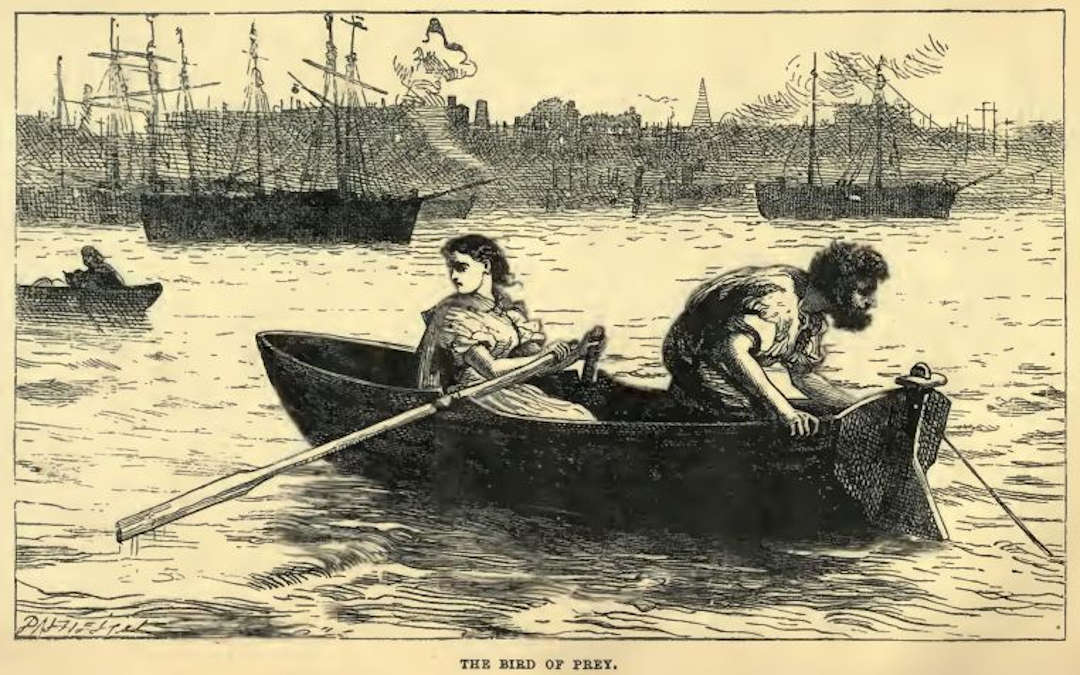
\includegraphics[scale=2.3]{01-01-01}

The figures in this boat were those of a strong man with ragged
grizzled hair and a sun-browned face, and a dark girl of nineteen or
twenty, sufficiently like him to be recognizable as his daughter.
The girl rowed, pulling a pair of sculls very easily; the man, with
the rudder-lines slack in his hands, and his hands loose in his
waistband, kept an eager look out. He had no net, hook, or line,
and he could not be a fisherman; his boat had no cushion for a
sitter, no paint, no inscription, no appliance beyond a rusty
boathook and a coil of rope, and he could not be a waterman; his
boat was too crazy and too small to take in cargo for delivery, and
he could not be a lighterman or river-carrier; there was no clue to
what he looked for, but he looked for something, with a most intent
and searching gaze. The tide, which had turned an hour before,
was running down, and his eyes watched every little race and eddy
in its broad sweep, as the boat made slight head-way against it, or
drove stern foremost before it, according as he directed his
daughter by a movement of his head. She watched his face as
earnestly as he watched the river. But, in the intensity of her look
there was a touch of dread or horror.

Allied to the bottom of the river rather than the surface, by reason
of the slime and ooze with which it was covered, and its sodden
state, this boat and the two figures in it obviously were doing
something that they often did, and were seeking what they often
sought. Half savage as the man showed, with no covering on his
matted head, with his brown arms bare to between the elbow and
the shoulder, with the loose knot of a looser kerchief lying low on
his bare breast in a wilderness of beard and whisker, with such
dress as he wore seeming to be made out of the mud that begrimed
his boat, still there was a business-like usage in his steady gaze.
So with every litle action of the girl, with every turn of her wrist,
perhaps most of all with her look of dread or horror; they were
things of usage.

'Keep her out, Lizzie. Tide runs strong here. Keep her well afore
the sweep of it.'

Trusting to the girl's skill and making no use of the rudder, he eyed
the coming tide with an absorbed attention. So the girl eyed him.
But, it happened now, that a slant of light from the setting sun
glanced into the bottom of the boat, and, touching a rotten stain
there which bore some resemblance to the outline of a muffled
human form, coloured it as though with diluted blood. This caught
the girl's eye, and she shivered.

'What ails you?' said the man, immediately aware of it, though so
intent on the advancing waters; 'I see nothing afloat.'

The red light was gone, the shudder was gone, and his gaze, which
had come back to the boat for a moment, travelled away again.
Wheresoever the strong tide met with an impediment, his gaze
paused for an instant. At every mooring-chain and rope, at every
stationery boat or barge that split the current into a broad-arrowhead,
at the offsets from the piers of Southwark Bridge, at the
paddles of the river steamboats as they beat the filthy water, at the
floating logs of timber lashed together lying off certain wharves,
his shining eyes darted a hungry look. After a darkening hour or
so, suddenly the rudder-lines tightened in his hold, and he steered
hard towards the Surrey shore.

Always watching his face, the girl instantly answered to the action
in her sculling; presently the boat swung round, quivered as from a
sudden jerk, and the upper half of the man was stretched out over
the stern.

The girl pulled the hood of a cloak she wore, over her head and
over her face, and, looking backward so that the front folds of this
hood were turned down the river, kept the boat in that direction
going before the tide.
Until now, the boat had barely held her own,
and had hovered about one spot; but now, the banks changed
swiftly, and the deepening shadows and the kindling lights of
London Bridge were passed, and the tiers of shipping lay on either
hand.

It was not until now that the upper half of the man came back into
the boat. His arms were wet and dirty, and he washed them over
the side. In his right hand he held something, and he washed that
in the river too.
It was money.
He chinked it once, and he blew
upon it once, and he spat upon it once,--'for luck,' he hoarsely said
--before he put it in his pocket.

'Lizzie!'

The girl turned her face towards him with a start, and rowed in silence.
Her face was very pale.
He was a hook-nosed man, and
with that and his bright eyes and his ruffled head, bore a certain
likeness to a roused bird of prey.

'Take that thing off your face.'

She put it back.

'Here! and give me hold of the sculls. I'll take the rest of the spell.'

'No, no, father! Father!--I cannot sit so near it!' No!
I can't indeed.

He was moving towards her to change places, but her terrified
expostulation stopped him and he resumed his seat.

‘What hurt can it do you?’

‘None, none. But I cannot bear it.’

‘It’s my belief you hate the sight of the very river.’

‘I--I do not like it, father.’

‘As if it wasn’t your living! As if it wasn’t meat and drink to you!’

At these latter words the girl shivered again, and for a moment paused
in her rowing, seeming to turn deadly faint. It escaped his attention,
for he was glancing over the stern at something the boat had in tow.

‘How can you be so thankless to your best friend, Lizzie? The very
fire that warmed you when you were a babby, was picked out of the river
alongside the coal barges. The very basket that you slept in, the tide
washed ashore. The very rockers that I put it upon to make a cradle
of it, I cut out of a piece of wood that drifted from some ship or
another.’

Lizzie took her right hand from the scull it held, and touched her
lips with it, and for a moment held it out lovingly towards him: then,
without speaking, she resumed her rowing, as another boat of similar
appearance, though in rather better trim, came out from a dark place and
dropped softly alongside.

‘In luck again, Gaffer?’ said a man with a squinting leer, who sculled
her and who was alone, ‘I know’d you was in luck again, by your wake as
you come down.’

‘Ah!’ replied the other, drily. ‘So you’re out, are you?’

‘Yes, pardner.’

There was now a tender yellow moonlight on the river, and the new comer,
keeping half his boat’s length astern of the other boat looked hard at
its track.

‘I says to myself,’ he went on, ‘directly you hove in view, yonder’s
Gaffer, and in luck again, by George if he ain’t! Scull it is,
pardner--don’t fret yourself--I didn’t touch him.’ This was in answer
to a quick impatient movement on the part of Gaffer: the speaker at the
same time unshipping his scull on that side, and laying his hand on the
gunwale of Gaffer’s boat and holding to it.

‘He’s had touches enough not to want no more, as well as I make him
out, Gaffer! Been a knocking about with a pretty many tides, ain’t he
pardner? Such is my out-of-luck ways, you see! He must have passed me
when he went up last time, for I was on the lookout below bridge here. I
a’most think you’re like the wulturs, pardner, and scent ‘em out.’

He spoke in a dropped voice, and with more than one glance at Lizzie who
had pulled on her hood again. Both men then looked with a weird unholy
interest in the wake of Gaffer’s boat.

‘Easy does it, betwixt us. Shall I take him aboard, pardner?’

‘No,’ said the other. In so surly a tone that the man, after a blank
stare, acknowledged it with the retort:

‘--Arn’t been eating nothing as has disagreed with you, have you,
pardner?’

‘Why, yes, I have,’ said Gaffer. ‘I have been swallowing too much of
that word, Pardner. I am no pardner of yours.’

‘Since when was you no pardner of mine, Gaffer Hexam Esquire?’

‘Since you was accused of robbing a man. Accused of robbing a live man!’
said Gaffer, with great indignation.

‘And what if I had been accused of robbing a dead man, Gaffer?’

‘You COULDN’T do it.’

‘Couldn’t you, Gaffer?’

‘No. Has a dead man any use for money? Is it possible for a dead man to
have money? What world does a dead man belong to? ‘Tother world. What
world does money belong to? This world. How can money be a corpse’s? Can
a corpse own it, want it, spend it, claim it, miss it? Don’t try to go
confounding the rights and wrongs of things in that way. But it’s worthy
of the sneaking spirit that robs a live man.’

‘I’ll tell you what it is--.’

‘No you won’t. I’ll tell you what it is. You got off with a short time
of it for putting your hand in the pocket of a sailor, a live sailor.
Make the most of it and think yourself lucky, but don’t think after
that to come over ME with your pardners. We have worked together in time
past, but we work together no more in time present nor yet future. Let
go. Cast off!’

‘Gaffer! If you think to get rid of me this way--.’

‘If I don’t get rid of you this way, I’ll try another, and chop you over
the fingers with the stretcher, or take a pick at your head with the
boat-hook. Cast off! Pull you, Lizzie. Pull home, since you won’t let
your father pull.’

Lizzie shot ahead, and the other boat fell astern. Lizzie’s father,
composing himself into the easy attitude of one who had asserted the
high moralities and taken an unassailable position, slowly lighted a
pipe, and smoked, and took a survey of what he had in tow. What he had
in tow, lunged itself at him sometimes in an awful manner when the boat
was checked, and sometimes seemed to try to wrench itself away, though
for the most part it followed submissively. A neophyte might have
fancied that the ripples passing over it were dreadfully like faint
changes of expression on a sightless face; but Gaffer was no neophyte
and had no fancies.


% REV00 Fri 26 Mar 2021 18:30:59 WIB
% START Fri 26 Mar 2021 18:30:49 WIB

\chapter{THE MAN FROM SOMEWHERE}

Mr and Mrs Veneering were bran-new people in a bran-new house in a
bran-new quarter of London. Everything about the Veneerings was spick
and span new. All their furniture was new, all their friends were new,
all their servants were new, their plate was new, their carriage was
new, their harness was new, their horses were new, their pictures
were new, they themselves were new, they were as newly married as was
lawfully compatible with their having a bran-new baby, and if they had
set up a great-grandfather, he would have come home in matting from the
Pantechnicon, without a scratch upon him, French polished to the crown
of his head.

For, in the Veneering establishment, from the hall-chairs with the new
coat of arms, to the grand pianoforte with the new action, and upstairs
again to the new fire-escape, all things were in a state of high varnish
and polish. And what was observable in the furniture, was observable in
the Veneerings--the surface smelt a little too much of the workshop and
was a trifle sticky.

There was an innocent piece of dinner-furniture that went upon easy
castors and was kept over a livery stable-yard in Duke Street, Saint
James’s, when not in use, to whom the Veneerings were a source of blind
confusion. The name of this article was Twemlow. Being first cousin
to Lord Snigsworth, he was in frequent requisition, and at many houses
might be said to represent the dining-table in its normal state. Mr and
Mrs Veneering, for example, arranging a dinner, habitually started with
Twemlow, and then put leaves in him, or added guests to him. Sometimes,
the table consisted of Twemlow and half a dozen leaves; sometimes, of
Twemlow and a dozen leaves; sometimes, Twemlow was pulled out to his
utmost extent of twenty leaves. Mr and Mrs Veneering on occasions of
ceremony faced each other in the centre of the board, and thus the
parallel still held; for, it always happened that the more Twemlow was
pulled out, the further he found himself from the center, and nearer
to the sideboard at one end of the room, or the window-curtains at the
other.

But, it was not this which steeped the feeble soul of Twemlow in
confusion. This he was used to, and could take soundings of. The abyss
to which he could find no bottom, and from which started forth the
engrossing and ever-swelling difficulty of his life, was the insoluble
question whether he was Veneering’s oldest friend, or newest friend.
To the excogitation of this problem, the harmless gentleman had devoted
many anxious hours, both in his lodgings over the livery stable-yard,
and in the cold gloom, favourable to meditation, of Saint James’s
Square. Thus. Twemlow had first known Veneering at his club, where
Veneering then knew nobody but the man who made them known to one
another, who seemed to be the most intimate friend he had in the world,
and whom he had known two days--the bond of union between their souls,
the nefarious conduct of the committee respecting the cookery of
a fillet of veal, having been accidentally cemented at that date.
Immediately upon this, Twemlow received an invitation to dine with
Veneering, and dined: the man being of the party. Immediately upon
that, Twemlow received an invitation to dine with the man, and dined:
Veneering being of the party. At the man’s were a Member, an Engineer, a
Payer-off of the National Debt, a Poem on Shakespeare, a Grievance, and
a Public Office, who all seem to be utter strangers to Veneering. And
yet immediately after that, Twemlow received an invitation to dine at
Veneerings, expressly to meet the Member, the Engineer, the Payer-off
of the National Debt, the Poem on Shakespeare, the Grievance, and the
Public Office, and, dining, discovered that all of them were the most
intimate friends Veneering had in the world, and that the wives of all
of them (who were all there) were the objects of Mrs Veneering’s most
devoted affection and tender confidence.

Thus it had come about, that Mr Twemlow had said to himself in his
lodgings, with his hand to his forehead: ‘I must not think of this. This
is enough to soften any man’s brain,’--and yet was always thinking of
it, and could never form a conclusion.

This evening the Veneerings give a banquet. Eleven leaves in the
Twemlow; fourteen in company all told. Four pigeon-breasted retainers in
plain clothes stand in line in the hall. A fifth retainer, proceeding up
the staircase with a mournful air--as who should say, ‘Here is another
wretched creature come to dinner; such is life!’--announces, ‘Mis-ter
Twemlow!’

Mrs Veneering welcomes her sweet Mr Twemlow. Mr Veneering welcomes
his dear Twemlow. Mrs Veneering does not expect that Mr Twemlow can in
nature care much for such insipid things as babies, but so old a friend
must please to look at baby. ‘Ah! You will know the friend of your
family better, Tootleums,’ says Mr Veneering, nodding emotionally at
that new article, ‘when you begin to take notice.’ He then begs to make
his dear Twemlow known to his two friends, Mr Boots and Mr Brewer--and
clearly has no distinct idea which is which.

But now a fearful circumstance occurs.

‘Mis-ter and Mis-sus Podsnap!’

‘My dear,’ says Mr Veneering to Mrs Veneering, with an air of much
friendly interest, while the door stands open, ‘the Podsnaps.’

A too, too smiling large man, with a fatal freshness on him, appearing
with his wife, instantly deserts his wife and darts at Twemlow with:

‘How do you do? So glad to know you. Charming house you have here. I
hope we are not late. So glad of the opportunity, I am sure!’

When the first shock fell upon him, Twemlow twice skipped back in
his neat little shoes and his neat little silk stockings of a bygone
fashion, as if impelled to leap over a sofa behind him; but the large
man closed with him and proved too strong.

‘Let me,’ says the large man, trying to attract the attention of his
wife in the distance, ‘have the pleasure of presenting Mrs Podsnap
to her host. She will be,’ in his fatal freshness he seems to find
perpetual verdure and eternal youth in the phrase, ‘she will be so glad
of the opportunity, I am sure!’

In the meantime, Mrs Podsnap, unable to originate a mistake on her own
account, because Mrs Veneering is the only other lady there, does her
best in the way of handsomely supporting her husband’s, by looking
towards Mr Twemlow with a plaintive countenance and remarking to Mrs
Veneering in a feeling manner, firstly, that she fears he has been
rather bilious of late, and, secondly, that the baby is already very
like him.

It is questionable whether any man quite relishes being mistaken for
any other man; but, Mr Veneering having this very evening set up the
shirt-front of the young Antinous in new worked cambric just come home,
is not at all complimented by being supposed to be Twemlow, who is dry
and weazen and some thirty years older. Mrs Veneering equally resents
the imputation of being the wife of Twemlow. As to Twemlow, he is
so sensible of being a much better bred man than Veneering, that he
considers the large man an offensive ass.

In this complicated dilemma, Mr Veneering approaches the large man with
extended hand and, smilingly assures that incorrigible personage that he
is delighted to see him: who in his fatal freshness instantly replies:

‘Thank you. I am ashamed to say that I cannot at this moment recall
where we met, but I am so glad of this opportunity, I am sure!’

Then pouncing upon Twemlow, who holds back with all his feeble might, he
is haling him off to present him, as Veneering, to Mrs Podsnap, when the
arrival of more guests unravels the mistake. Whereupon, having re-shaken
hands with Veneering as Veneering, he re-shakes hands with Twemlow as
Twemlow, and winds it all up to his own perfect satisfaction by saying
to the last-named, ‘Ridiculous opportunity--but so glad of it, I am
sure!’

Now, Twemlow having undergone this terrific experience, having likewise
noted the fusion of Boots in Brewer and Brewer in Boots, and having
further observed that of the remaining seven guests four discrete
characters enter with wandering eyes and wholly declined to commit
themselves as to which is Veneering, until Veneering has them in his
grasp;--Twemlow having profited by these studies, finds his brain
wholesomely hardening as he approaches the conclusion that he really is
Veneering’s oldest friend, when his brain softens again and all is
lost, through his eyes encountering Veneering and the large man linked
together as twin brothers in the back drawing-room near the conservatory
door, and through his ears informing him in the tones of Mrs Veneering
that the same large man is to be baby’s godfather.

‘Dinner is on the table!’

Thus the melancholy retainer, as who should say, ‘Come down and be
poisoned, ye unhappy children of men!’

Twemlow, having no lady assigned him, goes down in the rear, with
his hand to his forehead. Boots and Brewer, thinking him indisposed,
whisper, ‘Man faint. Had no lunch.’ But he is only stunned by the
unvanquishable difficulty of his existence.

Revived by soup, Twemlow discourses mildly of the Court Circular with
Boots and Brewer. Is appealed to, at the fish stage of the banquet, by
Veneering, on the disputed question whether his cousin Lord Snigsworth
is in or out of town? Gives it that his cousin is out of town. ‘At
Snigsworthy Park?’ Veneering inquires. ‘At Snigsworthy,’ Twemlow
rejoins. Boots and Brewer regard this as a man to be cultivated; and
Veneering is clear that he is a remunerative article. Meantime the
retainer goes round, like a gloomy Analytical Chemist: always seeming
to say, after ‘Chablis, sir?’--‘You wouldn’t if you knew what it’s made
of.’

The great looking-glass above the sideboard, reflects the table and the
company. Reflects the new Veneering crest, in gold and eke in silver,
frosted and also thawed, a camel of all work. The Heralds’ College found
out a Crusading ancestor for Veneering who bore a camel on his shield
(or might have done it if he had thought of it), and a caravan of camels
take charge of the fruits and flowers and candles, and kneel down be
loaded with the salt. Reflects Veneering; forty, wavy-haired, dark,
tending to corpulence, sly, mysterious, filmy--a kind of sufficiently
well-looking veiled-prophet, not prophesying. Reflects Mrs Veneering;
fair, aquiline-nosed and fingered, not so much light hair as she might
have, gorgeous in raiment and jewels, enthusiastic, propitiatory,
conscious that a corner of her husband’s veil is over herself. Reflects
Podsnap; prosperously feeding, two little light-coloured wiry wings, one
on either side of his else bald head, looking as like his hairbrushes as
his hair, dissolving view of red beads on his forehead, large allowance
of crumpled shirt-collar up behind. Reflects Mrs Podsnap; fine woman
for Professor Owen, quantity of bone, neck and nostrils like a
rocking-horse, hard features, majestic head-dress in which Podsnap has
hung golden offerings. Reflects Twemlow; grey, dry, polite, susceptible
to east wind, First-Gentleman-in-Europe collar and cravat, cheeks drawn
in as if he had made a great effort to retire into himself some years
ago, and had got so far and had never got any farther. Reflects mature
young lady; raven locks, and complexion that lights up well when well
powdered--as it is--carrying on considerably in the captivation of
mature young gentleman; with too much nose in his face, too much ginger
in his whiskers, too much torso in his waistcoat, too much sparkle in
his studs, his eyes, his buttons, his talk, and his teeth. Reflects
charming old Lady Tippins on Veneering’s right; with an immense obtuse
drab oblong face, like a face in a tablespoon, and a dyed Long Walk up
the top of her head, as a convenient public approach to the bunch of
false hair behind, pleased to patronize Mrs Veneering opposite, who
is pleased to be patronized. Reflects a certain ‘Mortimer’, another
of Veneering’s oldest friends; who never was in the house before,
and appears not to want to come again, who sits disconsolate on Mrs
Veneering’s left, and who was inveigled by Lady Tippins (a friend of
his boyhood) to come to these people’s and talk, and who won’t talk.
Reflects Eugene, friend of Mortimer; buried alive in the back of his
chair, behind a shoulder--with a powder-epaulette on it--of the mature
young lady, and gloomily resorting to the champagne chalice whenever
proffered by the Analytical Chemist. Lastly, the looking-glass reflects
Boots and Brewer, and two other stuffed Buffers interposed between the
rest of the company and possible accidents.

The Veneering dinners are excellent dinners--or new people wouldn’t
come--and all goes well. Notably, Lady Tippins has made a series of
experiments on her digestive functions, so extremely complicated and
daring, that if they could be published with their results it might
benefit the human race. Having taken in provisions from all parts of the
world, this hardy old cruiser has last touched at the North Pole, when,
as the ice-plates are being removed, the following words fall from her:

‘I assure you, my dear Veneering--’

(Poor Twemlow’s hand approaches his forehead, for it would seem now,
that Lady Tippins is going to be the oldest friend.)

‘I assure you, my dear Veneering, that it is the oddest affair! Like
the advertising people, I don’t ask you to trust me, without offering
a respectable reference. Mortimer there, is my reference, and knows all
about it.’

Mortimer raises his drooping eyelids, and slightly opens his mouth. But
a faint smile, expressive of ‘What’s the use!’ passes over his face, and
he drops his eyelids and shuts his mouth.

‘Now, Mortimer,’ says Lady Tippins, rapping the sticks of her closed
green fan upon the knuckles of her left hand--which is particularly rich
in knuckles, ‘I insist upon your telling all that is to be told about
the man from Jamaica.’

‘Give you my honour I never heard of any man from Jamaica, except the
man who was a brother,’ replies Mortimer.

‘Tobago, then.’

‘Nor yet from Tobago.’

‘Except,’ Eugene strikes in: so unexpectedly that the mature young lady,
who has forgotten all about him, with a start takes the epaulette out
of his way: ‘except our friend who long lived on rice-pudding and
isinglass, till at length to his something or other, his physician said
something else, and a leg of mutton somehow ended in daygo.’

A reviving impression goes round the table that Eugene is coming out. An
unfulfilled impression, for he goes in again.

‘Now, my dear Mrs Veneering,’ quoth Lady Tippins, I appeal to you
whether this is not the basest conduct ever known in this world? I carry
my lovers about, two or three at a time, on condition that they are very
obedient and devoted; and here is my oldest lover-in-chief, the head of
all my slaves, throwing off his allegiance before company! And here is
another of my lovers, a rough Cymon at present certainly, but of whom
I had most hopeful expectations as to his turning out well in course of
time, pretending that he can’t remember his nursery rhymes! On purpose
to annoy me, for he knows how I doat upon them!’

A grisly little fiction concerning her lovers is Lady Tippins’s point.
She is always attended by a lover or two, and she keeps a little list
of her lovers, and she is always booking a new lover, or striking out an
old lover, or putting a lover in her black list, or promoting a lover to
her blue list, or adding up her lovers, or otherwise posting her book.
Mrs Veneering is charmed by the humour, and so is Veneering. Perhaps it
is enhanced by a certain yellow play in Lady Tippins’s throat, like the
legs of scratching poultry.

‘I banish the false wretch from this moment, and I strike him out of
my Cupidon (my name for my Ledger, my dear,) this very night. But I am
resolved to have the account of the man from Somewhere, and I beg you
to elicit it for me, my love,’ to Mrs Veneering, ‘as I have lost my own
influence. Oh, you perjured man!’ This to Mortimer, with a rattle of her
fan.

‘We are all very much interested in the man from Somewhere,’ Veneering
observes.

Then the four Buffers, taking heart of grace all four at once, say:

‘Deeply interested!’

‘Quite excited!’

‘Dramatic!’

‘Man from Nowhere, perhaps!’

And then Mrs Veneering--for the Lady Tippins’s winning wiles are
contagious--folds her hands in the manner of a supplicating child, turns
to her left neighbour, and says, ‘Tease! Pay! Man from Tumwhere!’ At
which the four Buffers, again mysteriously moved all four at once,
explain, ‘You can’t resist!’

‘Upon my life,’ says Mortimer languidly, ‘I find it immensely
embarrassing to have the eyes of Europe upon me to this extent, and my
only consolation is that you will all of you execrate Lady Tippins in
your secret hearts when you find, as you inevitably will, the man from
Somewhere a bore. Sorry to destroy romance by fixing him with a local
habitation, but he comes from the place, the name of which escapes me,
but will suggest itself to everybody else here, where they make the
wine.’

Eugene suggests ‘Day and Martin’s.’

‘No, not that place,’ returns the unmoved Mortimer, ‘that’s where they
make the Port. My man comes from the country where they make the Cape
Wine. But look here, old fellow; its not at all statistical and it’s
rather odd.’

It is always noticeable at the table of the Veneerings, that no man
troubles himself much about the Veneerings themselves, and that any
one who has anything to tell, generally tells it to anybody else in
preference.

‘The man,’ Mortimer goes on, addressing Eugene, ‘whose name is Harmon,
was only son of a tremendous old rascal who made his money by Dust.’

‘Red velveteens and a bell?’ the gloomy Eugene inquires.

‘And a ladder and basket if you like. By which means, or by others, he
grew rich as a Dust Contractor, and lived in a hollow in a hilly country
entirely composed of Dust. On his own small estate the growling old
vagabond threw up his own mountain range, like an old volcano, and its
geological formation was Dust. Coal-dust, vegetable-dust, bone-dust,
crockery dust, rough dust and sifted dust,--all manner of Dust.’

A passing remembrance of Mrs Veneering, here induces Mortimer to address
his next half-dozen words to her; after which he wanders away again,
tries Twemlow and finds he doesn’t answer, ultimately takes up with the
Buffers who receive him enthusiastically.

‘The moral being--I believe that’s the right expression--of this
exemplary person, derived its highest gratification from anathematizing
his nearest relations and turning them out of doors. Having begun (as
was natural) by rendering these attentions to the wife of his bosom,
he next found himself at leisure to bestow a similar recognition on the
claims of his daughter. He chose a husband for her, entirely to his own
satisfaction and not in the least to hers, and proceeded to settle upon
her, as her marriage portion, I don’t know how much Dust, but something
immense. At this stage of the affair the poor girl respectfully
intimated that she was secretly engaged to that popular character whom
the novelists and versifiers call Another, and that such a marriage
would make Dust of her heart and Dust of her life--in short, would
set her up, on a very extensive scale, in her father’s business.
Immediately, the venerable parent--on a cold winter’s night, it is
said--anathematized and turned her out.’

Here, the Analytical Chemist (who has evidently formed a very low
opinion of Mortimer’s story) concedes a little claret to the Buffers;
who, again mysteriously moved all four at once, screw it slowly into
themselves with a peculiar twist of enjoyment, as they cry in chorus,
‘Pray go on.’

‘The pecuniary resources of Another were, as they usually are, of a very
limited nature. I believe I am not using too strong an expression when
I say that Another was hard up. However, he married the young lady, and
they lived in a humble dwelling, probably possessing a porch ornamented
with honeysuckle and woodbine twining, until she died. I must refer
you to the Registrar of the District in which the humble dwelling was
situated, for the certified cause of death; but early sorrow and anxiety
may have had to do with it, though they may not appear in the ruled
pages and printed forms. Indisputably this was the case with Another,
for he was so cut up by the loss of his young wife that if he outlived
her a year it was as much as he did.’

There is that in the indolent Mortimer, which seems to hint that if good
society might on any account allow itself to be impressible, he, one of
good society, might have the weakness to be impressed by what he here
relates. It is hidden with great pains, but it is in him. The gloomy
Eugene too, is not without some kindred touch; for, when that appalling
Lady Tippins declares that if Another had survived, he should have gone
down at the head of her list of lovers--and also when the mature young
lady shrugs her epaulettes, and laughs at some private and confidential
comment from the mature young gentleman--his gloom deepens to that
degree that he trifles quite ferociously with his dessert-knife.

Mortimer proceeds.

‘We must now return, as novelists say, and as we all wish they wouldn’t,
to the man from Somewhere. Being a boy of fourteen, cheaply educated
at Brussels when his sister’s expulsion befell, it was some little time
before he heard of it--probably from herself, for the mother was dead;
but that I don’t know. Instantly, he absconded, and came over here. He
must have been a boy of spirit and resource, to get here on a stopped
allowance of five sous a week; but he did it somehow, and he burst in
on his father, and pleaded his sister’s cause. Venerable parent promptly
resorts to anathematization, and turns him out. Shocked and terrified
boy takes flight, seeks his fortune, gets aboard ship, ultimately
turns up on dry land among the Cape wine: small proprietor, farmer,
grower--whatever you like to call it.’

At this juncture, shuffling is heard in the hall, and tapping is heard
at the dining-room door. Analytical Chemist goes to the door, confers
angrily with unseen tapper, appears to become mollified by descrying
reason in the tapping, and goes out.

‘So he was discovered, only the other day, after having been expatriated
about fourteen years.’

A Buffer, suddenly astounding the other three, by detaching himself, and
asserting individuality, inquires: ‘How discovered, and why?’

‘Ah! To be sure. Thank you for reminding me. Venerable parent dies.’

Same Buffer, emboldened by success, says: ‘When?’

‘The other day. Ten or twelve months ago.’

Same Buffer inquires with smartness, ‘What of?’ But herein perishes a
melancholy example; being regarded by the three other Buffers with a
stony stare, and attracting no further attention from any mortal.

‘Venerable parent,’ Mortimer repeats with a passing remembrance that
there is a Veneering at table, and for the first time addressing
him--‘dies.’

The gratified Veneering repeats, gravely, ‘dies’; and folds his arms,
and composes his brow to hear it out in a judicial manner, when he finds
himself again deserted in the bleak world.

‘His will is found,’ said Mortimer, catching Mrs Podsnap’s
rocking-horse’s eye. ‘It is dated very soon after the son’s flight. It
leaves the lowest of the range of dust-mountains, with some sort of a
dwelling-house at its foot, to an old servant who is sole executor, and
all the rest of the property--which is very considerable--to the son.
He directs himself to be buried with certain eccentric ceremonies and
precautions against his coming to life, with which I need not bore you,
and that’s all--except--’ and this ends the story.

The Analytical Chemist returning, everybody looks at him. Not because
anybody wants to see him, but because of that subtle influence in nature
which impels humanity to embrace the slightest opportunity of looking at
anything, rather than the person who addresses it.

‘--Except that the son’s inheriting is made conditional on his marrying
a girl, who at the date of the will, was a child of four or five years
old, and who is now a marriageable young woman. Advertisement and
inquiry discovered the son in the man from Somewhere, and at the present
moment, he is on his way home from there--no doubt, in a state of great
astonishment--to succeed to a very large fortune, and to take a wife.’

Mrs Podsnap inquires whether the young person is a young person of
personal charms? Mortimer is unable to report.

Mr Podsnap inquires what would become of the very large fortune, in the
event of the marriage condition not being fulfilled? Mortimer replies,
that by special testamentary clause it would then go to the old servant
above mentioned, passing over and excluding the son; also, that if
the son had not been living, the same old servant would have been sole
residuary legatee.

Mrs Veneering has just succeeded in waking Lady Tippins from a snore, by
dexterously shunting a train of plates and dishes at her knuckles across
the table; when everybody but Mortimer himself becomes aware that the
Analytical Chemist is, in a ghostly manner, offering him a folded paper.
Curiosity detains Mrs Veneering a few moments.

Mortimer, in spite of all the arts of the chemist, placidly refreshes
himself with a glass of Madeira, and remains unconscious of the Document
which engrosses the general attention, until Lady Tippins (who has a
habit of waking totally insensible), having remembered where she is, and
recovered a perception of surrounding objects, says: ‘Falser man than
Don Juan; why don’t you take the note from the commendatore?’ Upon
which, the chemist advances it under the nose of Mortimer, who looks
round at him, and says:

‘What’s this?’

Analytical Chemist bends and whispers.

‘WHO?’ Says Mortimer.

Analytical Chemist again bends and whispers.

Mortimer stares at him, and unfolds the paper. Reads it, reads it twice,
turns it over to look at the blank outside, reads it a third time.

‘This arrives in an extraordinarily opportune manner,’ says Mortimer
then, looking with an altered face round the table: ‘this is the
conclusion of the story of the identical man.’

‘Already married?’ one guesses.

‘Declines to marry?’ another guesses.

‘Codicil among the dust?’ another guesses.

‘Why, no,’ says Mortimer; ‘remarkable thing, you are all wrong. The
story is completer and rather more exciting than I supposed. Man’s
drowned!’



% REV00 Sat 27 Mar 2021 06:04:30 WIB
% START Sat 27 Mar 2021 06:04:30 WIB

\chapter{ANOTHER MAN}

As the disappearing skirts of the ladies ascended the Veneering
staircase, Mortimer, following them forth from the dining-room, turned
into a library of bran-new books, in bran-new bindings liberally gilded,
and requested to see the messenger who had brought the paper. He was a
boy of about fifteen. Mortimer looked at the boy, and the boy looked
at the bran-new pilgrims on the wall, going to Canterbury in more gold
frame than procession, and more carving than country.

‘Whose writing is this?’

‘Mine, sir.’

‘Who told you to write it?’

‘My father, Jesse Hexam.’

‘Is it he who found the body?’

‘Yes, sir.’

‘What is your father?’

The boy hesitated, looked reproachfully at the pilgrims as if they had
involved him in a little difficulty, then said, folding a plait in the
right leg of his trousers, ‘He gets his living along-shore.’

‘Is it far?’

‘Is which far?’ asked the boy, upon his guard, and again upon the road
to Canterbury.

‘To your father’s?’

‘It’s a goodish stretch, sir. I come up in a cab, and the cab’s waiting
to be paid. We could go back in it before you paid it, if you liked.
I went first to your office, according to the direction of the papers
found in the pockets, and there I see nobody but a chap of about my age
who sent me on here.’

There was a curious mixture in the boy, of uncompleted savagery, and
uncompleted civilization. His voice was hoarse and coarse, and his face
was coarse, and his stunted figure was coarse; but he was cleaner than
other boys of his type; and his writing, though large and round,
was good; and he glanced at the backs of the books, with an awakened
curiosity that went below the binding. No one who can read, ever looks
at a book, even unopened on a shelf, like one who cannot.

‘Were any means taken, do you know, boy, to ascertain if it was possible
to restore life?’ Mortimer inquired, as he sought for his hat.

‘You wouldn’t ask, sir, if you knew his state. Pharaoh’s multitude that
were drowned in the Red Sea, ain’t more beyond restoring to life. If
Lazarus was only half as far gone, that was the greatest of all the
miracles.’

‘Halloa!’ cried Mortimer, turning round with his hat upon his head, ‘you
seem to be at home in the Red Sea, my young friend?’

‘Read of it with teacher at the school,’ said the boy.

‘And Lazarus?’

‘Yes, and him too. But don’t you tell my father! We should have no peace
in our place, if that got touched upon. It’s my sister’s contriving.’

‘You seem to have a good sister.’

‘She ain’t half bad,’ said the boy; ‘but if she knows her letters it’s
the most she does--and them I learned her.’

The gloomy Eugene, with his hands in his pockets, had strolled in and
assisted at the latter part of the dialogue; when the boy spoke these
words slightingly of his sister, he took him roughly enough by the chin,
and turned up his face to look at it.

‘Well, I’m sure, sir!’ said the boy, resisting; ‘I hope you’ll know me
again.’

Eugene vouchsafed no answer; but made the proposal to Mortimer, ‘I’ll
go with you, if you like?’ So, they all three went away together in the
vehicle that had brought the boy; the two friends (once boys together at
a public school) inside, smoking cigars; the messenger on the box beside
the driver.

‘Let me see,’ said Mortimer, as they went along; ‘I have been, Eugene,
upon the honourable roll of solicitors of the High Court of Chancery,
and attorneys at Common Law, five years; and--except gratuitously taking
instructions, on an average once a fortnight, for the will of Lady
Tippins who has nothing to leave--I have had no scrap of business but
this romantic business.’

‘And I,’ said Eugene, ‘have been “called” seven years, and have had no
business at all, and never shall have any. And if I had, I shouldn’t
know how to do it.’

‘I am far from being clear as to the last particular,’ returned
Mortimer, with great composure, ‘that I have much advantage over you.’

‘I hate,’ said Eugene, putting his legs up on the opposite seat, ‘I hate
my profession.’

‘Shall I incommode you, if I put mine up too?’ returned Mortimer. ‘Thank
you. I hate mine.’

‘It was forced upon me,’ said the gloomy Eugene, ‘because it was
understood that we wanted a barrister in the family. We have got a
precious one.’

‘It was forced upon me,’ said Mortimer, ‘because it was understood that
we wanted a solicitor in the family. And we have got a precious one.’

‘There are four of us, with our names painted on a door-post in right of
one black hole called a set of chambers,’ said Eugene; ‘and each of us
has the fourth of a clerk--Cassim Baba, in the robber’s cave--and Cassim
is the only respectable member of the party.’

‘I am one by myself, one,’ said Mortimer, ‘high up an awful staircase
commanding a burial-ground, and I have a whole clerk to myself, and he
has nothing to do but look at the burial-ground, and what he will turn
out when arrived at maturity, I cannot conceive. Whether, in that shabby
rook’s nest, he is always plotting wisdom, or plotting murder; whether
he will grow up, after so much solitary brooding, to enlighten his
fellow-creatures, or to poison them; is the only speck of interest that
presents itself to my professional view. Will you give me a light? Thank
you.’

‘Then idiots talk,’ said Eugene, leaning back, folding his arms, smoking
with his eyes shut, and speaking slightly through his nose, ‘of Energy.
If there is a word in the dictionary under any letter from A to Z that
I abominate, it is energy. It is such a conventional superstition, such
parrot gabble! What the deuce! Am I to rush out into the street, collar
the first man of a wealthy appearance that I meet, shake him, and say,
“Go to law upon the spot, you dog, and retain me, or I’ll be the death
of you”? Yet that would be energy.’

‘Precisely my view of the case, Eugene. But show me a good opportunity,
show me something really worth being energetic about, and I’ll show you
energy.’

‘And so will I,’ said Eugene.

And it is likely enough that ten thousand other young men, within the
limits of the London Post-office town delivery, made the same hopeful
remark in the course of the same evening.

The wheels rolled on, and rolled down by the Monument and by the Tower,
and by the Docks; down by Ratcliffe, and by Rotherhithe; down by where
accumulated scum of humanity seemed to be washed from higher grounds,
like so much moral sewage, and to be pausing until its own weight forced
it over the bank and sunk it in the river. In and out among vessels
that seemed to have got ashore, and houses that seemed to have got
afloat--among bow-splits staring into windows, and windows staring
into ships--the wheels rolled on, until they stopped at a dark corner,
river-washed and otherwise not washed at all, where the boy alighted and
opened the door.

‘You must walk the rest, sir; it’s not many yards.’ He spoke in the
singular number, to the express exclusion of Eugene.

‘This is a confoundedly out-of-the-way place,’ said Mortimer, slipping
over the stones and refuse on the shore, as the boy turned the corner
sharp.

‘Here’s my father’s, sir; where the light is.’

The low building had the look of having once been a mill. There was a
rotten wart of wood upon its forehead that seemed to indicate where
the sails had been, but the whole was very indistinctly seen in the
obscurity of the night. The boy lifted the latch of the door, and they
passed at once into a low circular room, where a man stood before a red
fire, looking down into it, and a girl sat engaged in needlework. The
fire was in a rusty brazier, not fitted to the hearth; and a common
lamp, shaped like a hyacinth-root, smoked and flared in the neck of a
stone bottle on the table. There was a wooden bunk or berth in a corner,
and in another corner a wooden stair leading above--so clumsy and steep
that it was little better than a ladder. Two or three old sculls and
oars stood against the wall, and against another part of the wall was a
small dresser, making a spare show of the commonest articles of crockery
and cooking-vessels. The roof of the room was not plastered, but was
formed of the flooring of the room above. This, being very old, knotted,
seamed, and beamed, gave a lowering aspect to the chamber; and roof, and
walls, and floor, alike abounding in old smears of flour, red-lead (or
some such stain which it had probably acquired in warehousing), and
damp, alike had a look of decomposition.

‘The gentleman, father.’

The figure at the red fire turned, raised its ruffled head, and looked
like a bird of prey.

‘You’re Mortimer Lightwood Esquire; are you, sir?’

‘Mortimer Lightwood is my name. What you found,’ said Mortimer, glancing
rather shrinkingly towards the bunk; ‘is it here?’

‘’Tain’t not to say here, but it’s close by. I do everything reg’lar.
I’ve giv’ notice of the circumstarnce to the police, and the police have
took possession of it. No time ain’t been lost, on any hand. The police
have put into print already, and here’s what the print says of it.’

Taking up the bottle with the lamp in it, he held it near a paper on
the wall, with the police heading, BODY FOUND. The two friends read the
handbill as it stuck against the wall, and Gaffer read them as he held
the light.

‘Only papers on the unfortunate man, I see,’ said Lightwood, glancing
from the description of what was found, to the finder.

‘Only papers.’

Here the girl arose with her work in her hand, and went out at the door.

‘No money,’ pursued Mortimer; ‘but threepence in one of the
skirt-pockets.’

‘Three. Penny. Pieces,’ said Gaffer Hexam, in as many sentences.

‘The trousers pockets empty, and turned inside out.’

Gaffer Hexam nodded. ‘But that’s common. Whether it’s the wash of the
tide or no, I can’t say. Now, here,’ moving the light to another similar
placard, ‘HIS pockets was found empty, and turned inside out. And here,’
moving the light to another, ‘HER pocket was found empty, and turned
inside out. And so was this one’s. And so was that one’s. I can’t read,
nor I don’t want to it, for I know ‘em by their places on the wall. This
one was a sailor, with two anchors and a flag and G. F. T. on his arm.
Look and see if he warn’t.’

‘Quite right.’

‘This one was the young woman in grey boots, and her linen marked with a
cross. Look and see if she warn’t.’

‘Quite right.’

‘This is him as had a nasty cut over the eye. This is them two young
sisters what tied themselves together with a handkecher. This the
drunken old chap, in a pair of list slippers and a nightcap, wot had
offered--it afterwards come out--to make a hole in the water for a
quartern of rum stood aforehand, and kept to his word for the first and
last time in his life. They pretty well papers the room, you see; but I
know ‘em all. I’m scholar enough!’

He waved the light over the whole, as if to typify the light of his
scholarly intelligence, and then put it down on the table and stood
behind it looking intently at his visitors. He had the special
peculiarity of some birds of prey, that when he knitted his brow, his
ruffled crest stood highest.

‘You did not find all these yourself; did you?’ asked Eugene.

To which the bird of prey slowly rejoined, ‘And what might YOUR name be,
now?’

‘This is my friend,’ Mortimer Lightwood interposed; ‘Mr Eugene
Wrayburn.’

‘Mr Eugene Wrayburn, is it? And what might Mr Eugene Wrayburn have asked
of me?’

‘I asked you, simply, if you found all these yourself?’

‘I answer you, simply, most on ‘em.’

‘Do you suppose there has been much violence and robbery, beforehand,
among these cases?’

‘I don’t suppose at all about it,’ returned Gaffer. ‘I ain’t one of the
supposing sort. If you’d got your living to haul out of the river every
day of your life, you mightn’t be much given to supposing. Am I to show
the way?’

As he opened the door, in pursuance of a nod from Lightwood, an
extremely pale and disturbed face appeared in the doorway--the face of a
man much agitated.

‘A body missing?’ asked Gaffer Hexam, stopping short; ‘or a body found?
Which?’

‘I am lost!’ replied the man, in a hurried and an eager manner.

‘Lost?’

‘I--I--am a stranger, and don’t know the way. I--I--want to find the
place where I can see what is described here. It is possible I may know
it.’ He was panting, and could hardly speak; but, he showed a copy of
the newly-printed bill that was still wet upon the wall. Perhaps its
newness, or perhaps the accuracy of his observation of its general look,
guided Gaffer to a ready conclusion.

‘This gentleman, Mr Lightwood, is on that business.’

‘Mr Lightwood?’

During a pause, Mortimer and the stranger confronted each other. Neither
knew the other.

‘I think, sir,’ said Mortimer, breaking the awkward silence with his
airy self-possession, ‘that you did me the honour to mention my name?’

‘I repeated it, after this man.’

‘You said you were a stranger in London?’

‘An utter stranger.’

‘Are you seeking a Mr Harmon?’

‘No.’

‘Then I believe I can assure you that you are on a fruitless errand, and
will not find what you fear to find. Will you come with us?’

A little winding through some muddy alleys that might have been
deposited by the last ill-savoured tide, brought them to the
wicket-gate and bright lamp of a Police Station; where they found the
Night-Inspector, with a pen and ink, and ruler, posting up his books in
a whitewashed office, as studiously as if he were in a monastery on
top of a mountain, and no howling fury of a drunken woman were banging
herself against a cell-door in the back-yard at his elbow. With the
same air of a recluse much given to study, he desisted from his books to
bestow a distrustful nod of recognition upon Gaffer, plainly importing,
‘Ah! we know all about YOU, and you’ll overdo it some day;’ and to
inform Mr Mortimer Lightwood and friends, that he would attend them
immediately. Then, he finished ruling the work he had in hand (it might
have been illuminating a missal, he was so calm), in a very neat and
methodical manner, showing not the slightest consciousness of the woman
who was banging herself with increased violence, and shrieking most
terrifically for some other woman’s liver.

‘A bull’s-eye,’ said the Night-Inspector, taking up his keys. Which a
deferential satellite produced. ‘Now, gentlemen.’

With one of his keys, he opened a cool grot at the end of the yard,
and they all went in. They quickly came out again, no one speaking but
Eugene: who remarked to Mortimer, in a whisper, ‘Not MUCH worse than
Lady Tippins.’

So, back to the whitewashed library of the monastery--with that liver
still in shrieking requisition, as it had been loudly, while they looked
at the silent sight they came to see--and there through the merits of
the case as summed up by the Abbot. No clue to how body came into river.
Very often was no clue. Too late to know for certain, whether injuries
received before or after death; one excellent surgical opinion said,
before; other excellent surgical opinion said, after. Steward of ship in
which gentleman came home passenger, had been round to view, and could
swear to identity. Likewise could swear to clothes. And then, you
see, you had the papers, too. How was it he had totally disappeared on
leaving ship, ‘till found in river? Well! Probably had been upon some
little game. Probably thought it a harmless game, wasn’t up to things,
and it turned out a fatal game. Inquest to-morrow, and no doubt open
verdict.

‘It appears to have knocked your friend over--knocked him completely off
his legs,’ Mr Inspector remarked, when he had finished his summing up.
‘It has given him a bad turn to be sure!’ This was said in a very low
voice, and with a searching look (not the first he had cast) at the
stranger.

Mr Lightwood explained that it was no friend of his.

‘Indeed?’ said Mr Inspector, with an attentive ear; ‘where did you pick
him up?’

Mr Lightwood explained further.

Mr Inspector had delivered his summing up, and had added these words,
with his elbows leaning on his desk, and the fingers and thumb of his
right hand, fitting themselves to the fingers and thumb of his left.
Mr Inspector moved nothing but his eyes, as he now added, raising his
voice:

‘Turned you faint, sir! Seems you’re not accustomed to this kind of
work?’

The stranger, who was leaning against the chimneypiece with drooping
head, looked round and answered, ‘No. It’s a horrible sight!’

‘You expected to identify, I am told, sir?’

‘Yes.’

‘HAVE you identified?’

‘No. It’s a horrible sight. O! a horrible, horrible sight!’

‘Who did you think it might have been?’ asked Mr Inspector. ‘Give us a
description, sir. Perhaps we can help you.’

‘No, no,’ said the stranger; ‘it would be quite useless. Good-night.’

Mr Inspector had not moved, and had given no order; but, the satellite
slipped his back against the wicket, and laid his left arm along the top
of it, and with his right hand turned the bull’s-eye he had taken from
his chief--in quite a casual manner--towards the stranger.

‘You missed a friend, you know; or you missed a foe, you know; or you
wouldn’t have come here, you know. Well, then; ain’t it reasonable to
ask, who was it?’ Thus, Mr Inspector.

‘You must excuse my telling you. No class of man can understand better
than you, that families may not choose to publish their disagreements
and misfortunes, except on the last necessity. I do not dispute that you
discharge your duty in asking me the question; you will not dispute my
right to withhold the answer. Good-night.’

Again he turned towards the wicket, where the satellite, with his eye
upon his chief, remained a dumb statue.

‘At least,’ said Mr Inspector, ‘you will not object to leave me your
card, sir?’

‘I should not object, if I had one; but I have not.’ He reddened and was
much confused as he gave the answer.

‘At least,’ said Mr Inspector, with no change of voice or manner, ‘you
will not object to write down your name and address?’

‘Not at all.’

Mr Inspector dipped a pen in his inkstand, and deftly laid it on a
piece of paper close beside him; then resumed his former attitude.
The stranger stepped up to the desk, and wrote in a rather tremulous
hand--Mr Inspector taking sidelong note of every hair of his head when
it was bent down for the purpose--‘Mr Julius Handford, Exchequer Coffee
House, Palace Yard, Westminster.’

‘Staying there, I presume, sir?’

‘Staying there.’

‘Consequently, from the country?’

‘Eh? Yes--from the country.’

‘Good-night, sir.’

The satellite removed his arm and opened the wicket, and Mr Julius
Handford went out.

‘Reserve!’ said Mr Inspector. ‘Take care of this piece of paper, keep
him in view without giving offence, ascertain that he IS staying there,
and find out anything you can about him.’

The satellite was gone; and Mr Inspector, becoming once again the quiet
Abbot of that Monastery, dipped his pen in his ink and resumed
his books. The two friends who had watched him, more amused by the
professional manner than suspicious of Mr Julius Handford, inquired
before taking their departure too whether he believed there was anything
that really looked bad here?

The Abbot replied with reticence, couldn’t say. If a murder, anybody
might have done it. Burglary or pocket-picking wanted ‘prenticeship. Not
so, murder. We were all of us up to that. Had seen scores of people come
to identify, and never saw one person struck in that particular way.
Might, however, have been Stomach and not Mind. If so, rum stomach.
But to be sure there were rum everythings. Pity there was not a word
of truth in that superstition about bodies bleeding when touched by the
hand of the right person; you never got a sign out of bodies. You got
row enough out of such as her--she was good for all night now (referring
here to the banging demands for the liver), ‘but you got nothing out of
bodies if it was ever so.’

There being nothing more to be done until the Inquest was held next day,
the friends went away together, and Gaffer Hexam and his son went their
separate way. But, arriving at the last corner, Gaffer bade his boy go
home while he turned into a red-curtained tavern, that stood dropsically
bulging over the causeway, ‘for a half-a-pint.’

The boy lifted the latch he had lifted before, and found his sister
again seated before the fire at her work. Who raised her head upon his
coming in and asking:

‘Where did you go, Liz?’

‘I went out in the dark.’

‘There was no necessity for that. It was all right enough.’

‘One of the gentlemen, the one who didn’t speak while I was there,
looked hard at me. And I was afraid he might know what my face meant.
But there! Don’t mind me, Charley! I was all in a tremble of another
sort when you owned to father you could write a little.’

‘Ah! But I made believe I wrote so badly, as that it was odds if any one
could read it. And when I wrote slowest and smeared but with my finger
most, father was best pleased, as he stood looking over me.’

The girl put aside her work, and drawing her seat close to his seat by
the fire, laid her arm gently on his shoulder.

‘You’ll make the most of your time, Charley; won’t you?’

‘Won’t I? Come! I like that. Don’t I?’

‘Yes, Charley, yes. You work hard at your learning, I know. And I work
a little, Charley, and plan and contrive a little (wake out of my
sleep contriving sometimes), how to get together a shilling now, and a
shilling then, that shall make father believe you are beginning to earn
a stray living along shore.’

‘You are father’s favourite, and can make him believe anything.’

‘I wish I could, Charley! For if I could make him believe that learning
was a good thing, and that we might lead better lives, I should be
a’most content to die.’

‘Don’t talk stuff about dying, Liz.’

She placed her hands in one another on his shoulder, and laying her
rich brown cheek against them as she looked down at the fire, went on
thoughtfully:

‘Of an evening, Charley, when you are at the school, and father’s--’

‘At the Six Jolly Fellowship Porters,’ the boy struck in, with a
backward nod of his head towards the public-house.

‘Yes. Then as I sit a-looking at the fire, I seem to see in the burning
coal--like where that glow is now--’

‘That’s gas, that is,’ said the boy, ‘coming out of a bit of a forest
that’s been under the mud that was under the water in the days of Noah’s
Ark. Look here! When I take the poker--so--and give it a dig--’

‘Don’t disturb it, Charley, or it’ll be all in a blaze. It’s that dull
glow near it, coming and going, that I mean. When I look at it of an
evening, it comes like pictures to me, Charley.’

‘Show us a picture,’ said the boy. ‘Tell us where to look.’

‘Ah! It wants my eyes, Charley.’

‘Cut away then, and tell us what your eyes make of it.’

‘Why, there are you and me, Charley, when you were quite a baby that
never knew a mother--’

‘Don’t go saying I never knew a mother,’ interposed the boy, ‘for I knew
a little sister that was sister and mother both.’

The girl laughed delightedly, and her eyes filled with pleasant tears,
as he put both his arms round her waist and so held her.

‘There are you and me, Charley, when father was away at work and locked
us out, for fear we should set ourselves afire or fall out of window,
sitting on the door-sill, sitting on other door-steps, sitting on the
bank of the river, wandering about to get through the time. You
are rather heavy to carry, Charley, and I am often obliged to rest.
Sometimes we are sleepy and fall asleep together in a corner, sometimes
we are very hungry, sometimes we are a little frightened, but what is
oftenest hard upon us is the cold. You remember, Charley?’

‘I remember,’ said the boy, pressing her to him twice or thrice, ‘that I
snuggled under a little shawl, and it was warm there.’

‘Sometimes it rains, and we creep under a boat or the like of that:
sometimes it’s dark, and we get among the gaslights, sitting watching
the people as they go along the streets. At last, up comes father and
takes us home. And home seems such a shelter after out of doors! And
father pulls my shoes off, and dries my feet at the fire, and has me
to sit by him while he smokes his pipe long after you are abed, and
I notice that father’s is a large hand but never a heavy one when it
touches me, and that father’s is a rough voice but never an angry one
when it speaks to me. So, I grow up, and little by little father trusts
me, and makes me his companion, and, let him be put out as he may, never
once strikes me.’

The listening boy gave a grunt here, as much as to say ‘But he strikes
ME though!’

‘Those are some of the pictures of what is past, Charley.’

‘Cut away again,’ said the boy, ‘and give us a fortune-telling one; a
future one.’

‘Well! There am I, continuing with father and holding to father, because
father loves me and I love father. I can’t so much as read a book,
because, if I had learned, father would have thought I was deserting
him, and I should have lost my influence. I have not the influence I
want to have, I cannot stop some dreadful things I try to stop, but I
go on in the hope and trust that the time will come. In the meanwhile
I know that I am in some things a stay to father, and that if I was
not faithful to him he would--in revenge-like, or in disappointment, or
both--go wild and bad.’

‘Give us a touch of the fortune-telling pictures about me.’

‘I was passing on to them, Charley,’ said the girl, who had not changed
her attitude since she began, and who now mournfully shook her head;
‘the others were all leading up. There are you--’

‘Where am I, Liz?’

‘Still in the hollow down by the flare.’

‘There seems to be the deuce-and-all in the hollow down by the flare,’
said the boy, glancing from her eyes to the brazier, which had a grisly
skeleton look on its long thin legs.

‘There are you, Charley, working your way, in secret from father, at
the school; and you get prizes; and you go on better and better; and you
come to be a--what was it you called it when you told me about that?’

‘Ha, ha! Fortune-telling not know the name!’ cried the boy, seeming to
be rather relieved by this default on the part of the hollow down by the
flare. ‘Pupil-teacher.’

‘You come to be a pupil-teacher, and you still go on better and better,
and you rise to be a master full of learning and respect. But the secret
has come to father’s knowledge long before, and it has divided you from
father, and from me.’

‘No it hasn’t!’

‘Yes it has, Charley. I see, as plain as plain can be, that your way is
not ours, and that even if father could be got to forgive your taking
it (which he never could be), that way of yours would be darkened by our
way. But I see too, Charley--’

‘Still as plain as plain can be, Liz?’ asked the boy playfully.

‘Ah! Still. That it is a great work to have cut you away from father’s
life, and to have made a new and good beginning. So there am I, Charley,
left alone with father, keeping him as straight as I can, watching
for more influence than I have, and hoping that through some fortunate
chance, or when he is ill, or when--I don’t know what--I may turn him to
wish to do better things.’

‘You said you couldn’t read a book, Lizzie. Your library of books is the
hollow down by the flare, I think.’

‘I should be very glad to be able to read real books. I feel my want of
learning very much, Charley. But I should feel it much more, if I didn’t
know it to be a tie between me and father.--Hark! Father’s tread!’

It being now past midnight, the bird of prey went straight to roost. At
mid-day following he reappeared at the Six Jolly Fellowship Porters, in
the character, not new to him, of a witness before a Coroner’s Jury.

Mr Mortimer Lightwood, besides sustaining the character of one of the
witnesses, doubled the part with that of the eminent solicitor who
watched the proceedings on behalf of the representatives of the
deceased, as was duly recorded in the newspapers. Mr Inspector watched
the proceedings too, and kept his watching closely to himself. Mr Julius
Handford having given his right address, and being reported in solvent
circumstances as to his bill, though nothing more was known of him at
his hotel except that his way of life was very retired, had no summons
to appear, and was merely present in the shades of Mr Inspector’s mind.

The case was made interesting to the public, by Mr Mortimer Lightwood’s
evidence touching the circumstances under which the deceased, Mr John
Harmon, had returned to England; exclusive private proprietorship in
which circumstances was set up at dinner-tables for several days, by
Veneering, Twemlow, Podsnap, and all the Buffers: who all related them
irreconcilably with one another, and contradicted themselves. It was
also made interesting by the testimony of Job Potterson, the ship’s
steward, and one Mr Jacob Kibble, a fellow-passenger, that the deceased
Mr John Harmon did bring over, in a hand-valise with which he did
disembark, the sum realized by the forced sale of his little landed
property, and that the sum exceeded, in ready money, seven hundred
pounds. It was further made interesting, by the remarkable experiences
of Jesse Hexam in having rescued from the Thames so many dead bodies,
and for whose behoof a rapturous admirer subscribing himself ‘A friend
to Burial’ (perhaps an undertaker), sent eighteen postage stamps, and
five ‘Now Sir’s to the editor of the Times.

Upon the evidence adduced before them, the Jury found, That the body
of Mr John Harmon had been discovered floating in the Thames, in an
advanced state of decay, and much injured; and that the said Mr John
Harmon had come by his death under highly suspicious circumstances,
though by whose act or in what precise manner there was no evidence
before this Jury to show. And they appended to their verdict, a
recommendation to the Home Office (which Mr Inspector appeared to think
highly sensible), to offer a reward for the solution of the mystery.
Within eight-and-forty hours, a reward of One Hundred Pounds was
proclaimed, together with a free pardon to any person or persons not the
actual perpetrator or perpetrators, and so forth in due form.

This Proclamation rendered Mr Inspector additionally studious, and
caused him to stand meditating on river-stairs and causeways, and to go
lurking about in boats, putting this and that together. But, according
to the success with which you put this and that together, you get a
woman and a fish apart, or a Mermaid in combination. And Mr Inspector
could turn out nothing better than a Mermaid, which no Judge and Jury
would believe in.

Thus, like the tides on which it had been borne to the knowledge of men,
the Harmon Murder--as it came to be popularly called--went up and down,
and ebbed and flowed, now in the town, now in the country, now among
palaces, now among hovels, now among lords and ladies and gentlefolks,
now among labourers and hammerers and ballast-heavers, until at last,
after a long interval of slack water it got out to sea and drifted away.



% REV00 Fri 26 Mar 2021 17:51:51 WIB
% START Fri 26 Mar 2021 17:51:51 WIB

\chapter{THE R. WILFER FAMILY}


Reginald Wilfer is a name with rather a grand sound, suggesting on
first acquaintance brasses in country churches, scrolls in stained-glass
windows, and generally the De Wilfers who came over with the Conqueror.
For, it is a remarkable fact in genealogy that no De Any ones ever came
over with Anybody else.

But, the Reginald Wilfer family were of such commonplace extraction and
pursuits that their forefathers had for generations modestly subsisted
on the Docks, the Excise Office, and the Custom House, and the existing
R. Wilfer was a poor clerk. So poor a clerk, though having a limited
salary and an unlimited family, that he had never yet attained the
modest object of his ambition: which was, to wear a complete new suit
of clothes, hat and boots included, at one time. His black hat was brown
before he could afford a coat, his pantaloons were white at the seams
and knees before he could buy a pair of boots, his boots had worn out
before he could treat himself to new pantaloons, and, by the time he
worked round to the hat again, that shining modern article roofed-in an
ancient ruin of various periods.

If the conventional Cherub could ever grow up and be clothed, he might
be photographed as a portrait of Wilfer. His chubby, smooth, innocent
appearance was a reason for his being always treated with condescension
when he was not put down. A stranger entering his own poor house at
about ten o’clock P.M. might have been surprised to find him sitting up
to supper. So boyish was he in his curves and proportions, that his
old schoolmaster meeting him in Cheapside, might have been unable to
withstand the temptation of caning him on the spot. In short, he was
the conventional cherub, after the supposititious shoot just mentioned,
rather grey, with signs of care on his expression, and in decidedly
insolvent circumstances.

He was shy, and unwilling to own to the name of Reginald, as being too
aspiring and self-assertive a name. In his signature he used only the
initial R., and imparted what it really stood for, to none but chosen
friends, under the seal of confidence. Out of this, the facetious habit
had arisen in the neighbourhood surrounding Mincing Lane of making
christian names for him of adjectives and participles beginning with R.
Some of these were more or less appropriate: as Rusty, Retiring, Ruddy,
Round, Ripe, Ridiculous, Ruminative; others, derived their point from
their want of application: as Raging, Rattling, Roaring, Raffish. But,
his popular name was Rumty, which in a moment of inspiration had been
bestowed upon him by a gentleman of convivial habits connected with the
drug-markets, as the beginning of a social chorus, his leading part in
the execution of which had led this gentleman to the Temple of Fame, and
of which the whole expressive burden ran:

     ‘Rumty iddity, row dow dow,
     Sing toodlely, teedlely, bow wow wow.’

Thus he was constantly addressed, even in minor notes on business, as
‘Dear Rumty’; in answer to which, he sedately signed himself, ‘Yours
truly, R. Wilfer.’

He was clerk in the drug-house of Chicksey, Veneering, and Stobbles.
Chicksey and Stobbles, his former masters, had both become absorbed in
Veneering, once their traveller or commission agent: who had signalized
his accession to supreme power by bringing into the business a quantity
of plate-glass window and French-polished mahogany partition, and a
gleaming and enormous doorplate.

R. Wilfer locked up his desk one evening, and, putting his bunch of keys
in his pocket much as if it were his peg-top, made for home. His home
was in the Holloway region north of London, and then divided from it by
fields and trees. Between Battle Bridge and that part of the Holloway
district in which he dwelt, was a tract of suburban Sahara, where tiles
and bricks were burnt, bones were boiled, carpets were beat, rubbish was
shot, dogs were fought, and dust was heaped by contractors. Skirting
the border of this desert, by the way he took, when the light of its
kiln-fires made lurid smears on the fog, R. Wilfer sighed and shook his
head.

‘Ah me!’ said he, ‘what might have been is not what is!’

With which commentary on human life, indicating an experience of it
not exclusively his own, he made the best of his way to the end of his
journey.

Mrs Wilfer was, of course, a tall woman and an angular. Her lord being
cherubic, she was necessarily majestic, according to the principle which
matrimonially unites contrasts. She was much given to tying up her head
in a pocket-handkerchief, knotted under the chin. This head-gear, in
conjunction with a pair of gloves worn within doors, she seemed to
consider as at once a kind of armour against misfortune (invariably
assuming it when in low spirits or difficulties), and as a species of
full dress. It was therefore with some sinking of the spirit that her
husband beheld her thus heroically attired, putting down her candle in
the little hall, and coming down the doorsteps through the little front
court to open the gate for him.

Something had gone wrong with the house-door, for R. Wilfer stopped on
the steps, staring at it, and cried:

‘Hal-loa?’

‘Yes,’ said Mrs Wilfer, ‘the man came himself with a pair of pincers,
and took it off, and took it away. He said that as he had no expectation
of ever being paid for it, and as he had an order for another LADIES’
SCHOOL door-plate, it was better (burnished up) for the interests of all
parties.’

‘Perhaps it was, my dear; what do you think?’

‘You are master here, R. W.,’ returned his wife. ‘It is as you think;
not as I do. Perhaps it might have been better if the man had taken the
door too?’

‘My dear, we couldn’t have done without the door.’

‘Couldn’t we?’

‘Why, my dear! Could we?’

‘It is as you think, R. W.; not as I do.’ With those submissive words,
the dutiful wife preceded him down a few stairs to a little basement
front room, half kitchen, half parlour, where a girl of about nineteen,
with an exceedingly pretty figure and face, but with an impatient and
petulant expression both in her face and in her shoulders (which in
her sex and at her age are very expressive of discontent), sat playing
draughts with a younger girl, who was the youngest of the House of
Wilfer. Not to encumber this page by telling off the Wilfers in detail
and casting them up in the gross, it is enough for the present that the
rest were what is called ‘out in the world,’ in various ways, and that
they were Many. So many, that when one of his dutiful children called in
to see him, R. Wilfer generally seemed to say to himself, after a little
mental arithmetic, ‘Oh! here’s another of ‘em!’ before adding aloud,
‘How de do, John,’ or Susan, as the case might be.

‘Well Piggywiggies,’ said R. W., ‘how de do to-night? What I was
thinking of, my dear,’ to Mrs Wilfer already seated in a corner with
folded gloves, ‘was, that as we have let our first floor so well, and as
we have now no place in which you could teach pupils even if pupils--’

‘The milkman said he knew of two young ladies of the highest
respectability who were in search of a suitable establishment, and he
took a card,’ interposed Mrs Wilfer, with severe monotony, as if she
were reading an Act of Parliament aloud. ‘Tell your father whether it
was last Monday, Bella.’

‘But we never heard any more of it, ma,’ said Bella, the elder girl.

‘In addition to which, my dear,’ her husband urged, ‘if you have no
place to put two young persons into--’

‘Pardon me,’ Mrs Wilfer again interposed; ‘they were not young persons.
Two young ladies of the highest respectability. Tell your father, Bella,
whether the milkman said so.’

‘My dear, it is the same thing.’

‘No it is not,’ said Mrs Wilfer, with the same impressive monotony.
‘Pardon me!’

‘I mean, my dear, it is the same thing as to space. As to space. If you
have no space in which to put two youthful fellow-creatures, however
eminently respectable, which I do not doubt, where are those youthful
fellow-creatures to be accommodated? I carry it no further than that.
And solely looking at it,’ said her husband, making the stipulation at
once in a conciliatory, complimentary, and argumentative tone--‘as I am
sure you will agree, my love--from a fellow-creature point of view, my
dear.’

‘I have nothing more to say,’ returned Mrs Wilfer, with a meek
renunciatory action of her gloves. ‘It is as you think, R. W.; not as I
do.’

Here, the huffing of Miss Bella and the loss of three of her men at a
swoop, aggravated by the coronation of an opponent, led to that young
lady’s jerking the draught-board and pieces off the table: which her
sister went down on her knees to pick up.

‘Poor Bella!’ said Mrs Wilfer.

‘And poor Lavinia, perhaps, my dear?’ suggested R. W.

‘Pardon me,’ said Mrs Wilfer, ‘no!’

It was one of the worthy woman’s specialities that she had an amazing
power of gratifying her splenetic or worldly-minded humours by extolling
her own family: which she thus proceeded, in the present case, to do.

‘No, R. W. Lavinia has not known the trial that Bella has known. The
trial that your daughter Bella has undergone, is, perhaps, without
a parallel, and has been borne, I will say, Nobly. When you see your
daughter Bella in her black dress, which she alone of all the family
wears, and when you remember the circumstances which have led to
her wearing it, and when you know how those circumstances have been
sustained, then, R. W., lay your head upon your pillow and say, “Poor
Lavinia!”’

Here, Miss Lavinia, from her kneeling situation under the table, put in
that she didn’t want to be ‘poored by pa’, or anybody else.

‘I am sure you do not, my dear,’ returned her mother, ‘for you have a
fine brave spirit. And your sister Cecilia has a fine brave spirit
of another kind, a spirit of pure devotion, a beau-ti-ful spirit! The
self-sacrifice of Cecilia reveals a pure and womanly character, very
seldom equalled, never surpassed. I have now in my pocket a letter from
your sister Cecilia, received this morning--received three months after
her marriage, poor child!--in which she tells me that her husband must
unexpectedly shelter under their roof his reduced aunt. “But I will be
true to him, mamma,” she touchingly writes, “I will not leave him, I
must not forget that he is my husband. Let his aunt come!” If this is
not pathetic, if this is not woman’s devotion--!’ The good lady waved
her gloves in a sense of the impossibility of saying more, and tied the
pocket-handkerchief over her head in a tighter knot under her chin.

Bella, who was now seated on the rug to warm herself, with her brown
eyes on the fire and a handful of her brown curls in her mouth, laughed
at this, and then pouted and half cried.

‘I am sure,’ said she, ‘though you have no feeling for me, pa, I am one
of the most unfortunate girls that ever lived. You know how poor we are’
(it is probable he did, having some reason to know it!), ‘and what a
glimpse of wealth I had, and how it melted away, and how I am here in
this ridiculous mourning--which I hate!--a kind of a widow who never was
married. And yet you don’t feel for me.--Yes you do, yes you do.’

This abrupt change was occasioned by her father’s face. She stopped
to pull him down from his chair in an attitude highly favourable to
strangulation, and to give him a kiss and a pat or two on the cheek.

‘But you ought to feel for me, you know, pa.’

‘My dear, I do.’

‘Yes, and I say you ought to. If they had only left me alone and told
me nothing about it, it would have mattered much less. But that nasty Mr
Lightwood feels it his duty, as he says, to write and tell me what is in
reserve for me, and then I am obliged to get rid of George Sampson.’

Here, Lavinia, rising to the surface with the last draughtman rescued,
interposed, ‘You never cared for George Sampson, Bella.’

‘And did I say I did, miss?’ Then, pouting again, with the curls in her
mouth; ‘George Sampson was very fond of me, and admired me very much,
and put up with everything I did to him.’

‘You were rude enough to him,’ Lavinia again interposed.

‘And did I say I wasn’t, miss? I am not setting up to be sentimental
about George Sampson. I only say George Sampson was better than
nothing.’

‘You didn’t show him that you thought even that,’ Lavinia again
interposed.

‘You are a chit and a little idiot,’ returned Bella, ‘or you wouldn’t
make such a dolly speech. What did you expect me to do? Wait till you
are a woman, and don’t talk about what you don’t understand. You only
show your ignorance!’ Then, whimpering again, and at intervals biting
the curls, and stopping to look how much was bitten off, ‘It’s a shame!
There never was such a hard case! I shouldn’t care so much if it wasn’t
so ridiculous. It was ridiculous enough to have a stranger coming over
to marry me, whether he liked it or not. It was ridiculous enough to
know what an embarrassing meeting it would be, and how we never
could pretend to have an inclination of our own, either of us. It was
ridiculous enough to know I shouldn’t like him--how COULD I like him,
left to him in a will, like a dozen of spoons, with everything cut and
dried beforehand, like orange chips. Talk of orange flowers indeed!
I declare again it’s a shame! Those ridiculous points would have been
smoothed away by the money, for I love money, and want money--want it
dreadfully. I hate to be poor, and we are degradingly poor, offensively
poor, miserably poor, beastly poor. But here I am, left with all the
ridiculous parts of the situation remaining, and, added to them all,
this ridiculous dress! And if the truth was known, when the Harmon
murder was all over the town, and people were speculating on its being
suicide, I dare say those impudent wretches at the clubs and places made
jokes about the miserable creature’s having preferred a watery grave to
me. It’s likely enough they took such liberties; I shouldn’t wonder! I
declare it’s a very hard case indeed, and I am a most unfortunate girl.
The idea of being a kind of a widow, and never having been married!
And the idea of being as poor as ever after all, and going into black,
besides, for a man I never saw, and should have hated--as far as HE was
concerned--if I had seen!’

The young lady’s lamentations were checked at this point by a knuckle,
knocking at the half-open door of the room. The knuckle had knocked two
or three times already, but had not been heard.

‘Who is it?’ said Mrs Wilfer, in her Act-of-Parliament manner. ‘Enter!’

A gentleman coming in, Miss Bella, with a short and sharp exclamation,
scrambled off the hearth-rug and massed the bitten curls together in
their right place on her neck.

‘The servant girl had her key in the door as I came up, and directed me
to this room, telling me I was expected. I am afraid I should have asked
her to announce me.’

‘Pardon me,’ returned Mrs Wilfer. ‘Not at all. Two of my daughters. R.
W., this is the gentleman who has taken your first-floor. He was so good
as to make an appointment for to-night, when you would be at home.’

A dark gentleman. Thirty at the utmost. An expressive, one might say
handsome, face. A very bad manner. In the last degree constrained,
reserved, diffident, troubled. His eyes were on Miss Bella for an
instant, and then looked at the ground as he addressed the master of the
house.

‘Seeing that I am quite satisfied, Mr Wilfer, with the rooms, and with
their situation, and with their price, I suppose a memorandum between us
of two or three lines, and a payment down, will bind the bargain? I wish
to send in furniture without delay.’

Two or three times during this short address, the cherub addressed had
made chubby motions towards a chair. The gentleman now took it, laying
a hesitating hand on a corner of the table, and with another hesitating
hand lifting the crown of his hat to his lips, and drawing it before his
mouth.

‘The gentleman, R. W.,’ said Mrs Wilfer, ‘proposes to take your
apartments by the quarter. A quarter’s notice on either side.’

‘Shall I mention, sir,’ insinuated the landlord, expecting it to be
received as a matter of course, ‘the form of a reference?’

‘I think,’ returned the gentleman, after a pause, ‘that a reference is
not necessary; neither, to say the truth, is it convenient, for I am
a stranger in London. I require no reference from you, and perhaps,
therefore, you will require none from me. That will be fair on both
sides. Indeed, I show the greater confidence of the two, for I will pay
in advance whatever you please, and I am going to trust my furniture
here. Whereas, if you were in embarrassed circumstances--this is merely
supposititious--’

Conscience causing R. Wilfer to colour, Mrs Wilfer, from a corner (she
always got into stately corners) came to the rescue with a deep-toned
‘Per-fectly.’

‘--Why then I--might lose it.’

‘Well!’ observed R. Wilfer, cheerfully, ‘money and goods are certainly
the best of references.’

‘Do you think they ARE the best, pa?’ asked Miss Bella, in a low voice,
and without looking over her shoulder as she warmed her foot on the
fender.

‘Among the best, my dear.’

‘I should have thought, myself, it was so easy to add the usual kind of
one,’ said Bella, with a toss of her curls.

The gentleman listened to her, with a face of marked attention, though
he neither looked up nor changed his attitude. He sat, still and silent,
until his future landlord accepted his proposals, and brought writing
materials to complete the business. He sat, still and silent, while the
landlord wrote.

When the agreement was ready in duplicate (the landlord having worked
at it like some cherubic scribe, in what is conventionally called a
doubtful, which means a not at all doubtful, Old Master), it was signed
by the contracting parties, Bella looking on as scornful witness. The
contracting parties were R. Wilfer, and John Rokesmith Esquire.

When it came to Bella’s turn to sign her name, Mr Rokesmith, who was
standing, as he had sat, with a hesitating hand upon the table, looked
at her stealthily, but narrowly. He looked at the pretty figure bending
down over the paper and saying, ‘Where am I to go, pa? Here, in this
corner?’ He looked at the beautiful brown hair, shading the coquettish
face; he looked at the free dash of the signature, which was a bold one
for a woman’s; and then they looked at one another.

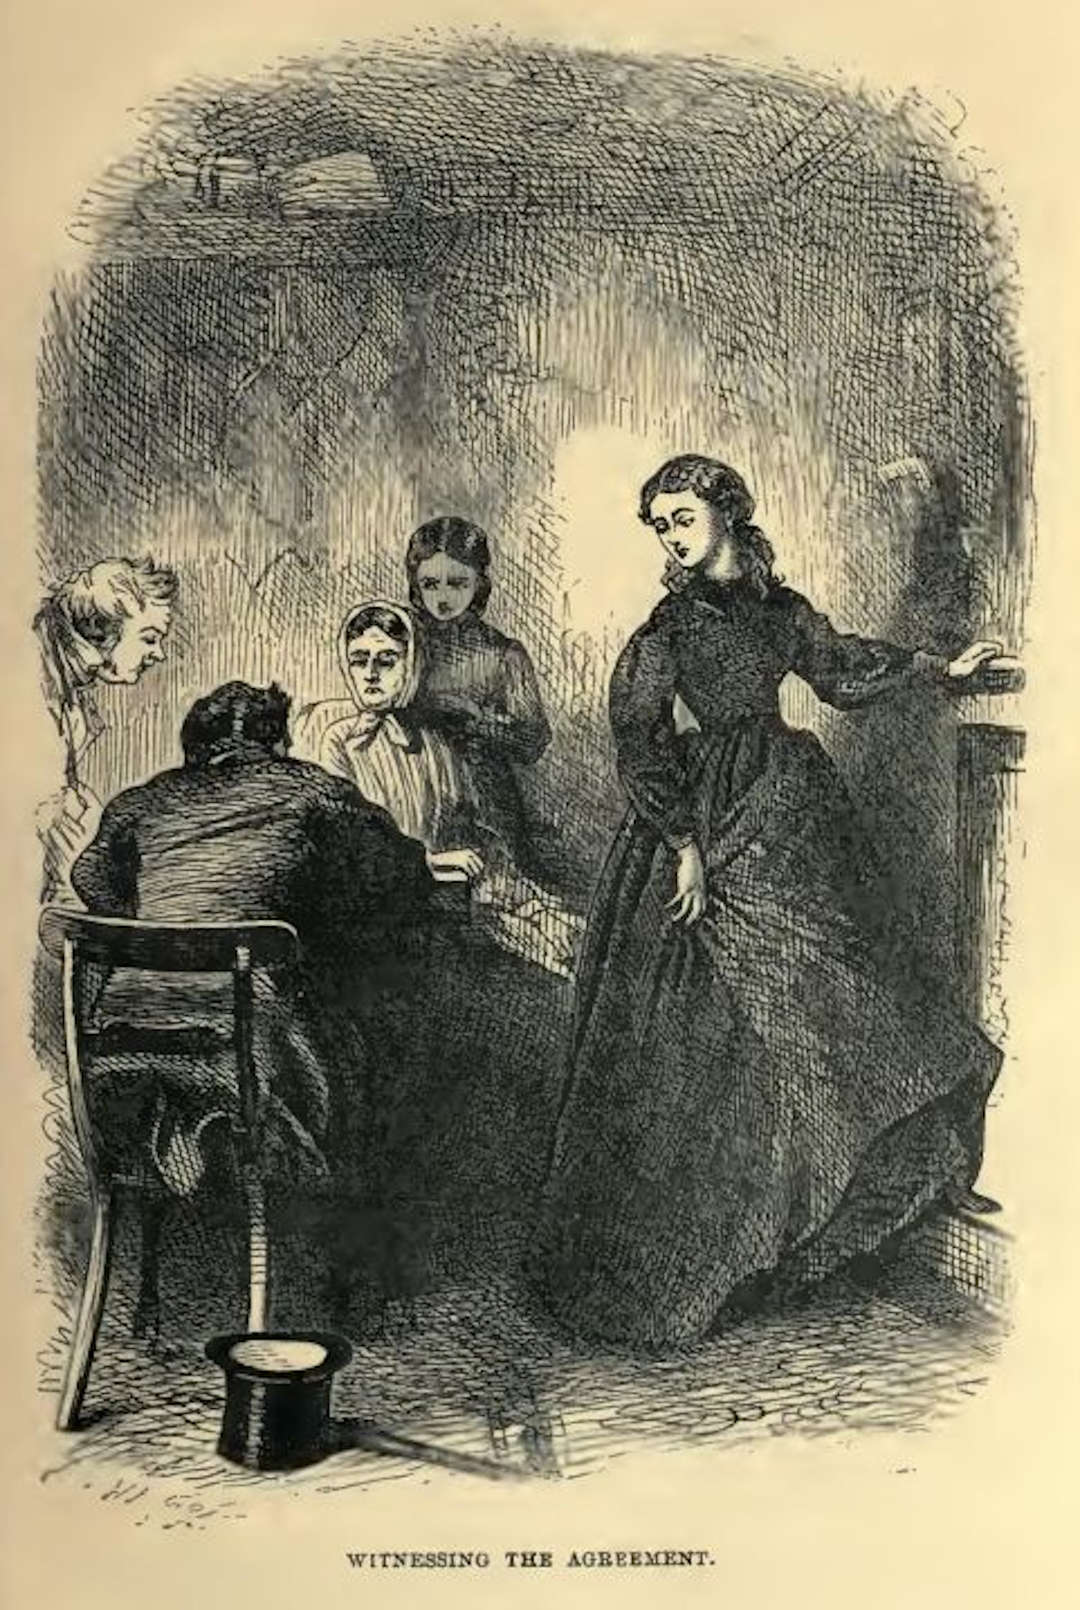
\includegraphics[scale=2.3]{01-04-01}

‘Much obliged to you, Miss Wilfer.’

‘Obliged?’

‘I have given you so much trouble.’

‘Signing my name? Yes, certainly. But I am your landlord’s daughter,
sir.’

As there was nothing more to do but pay eight sovereigns in earnest of
the bargain, pocket the agreement, appoint a time for the arrival of his
furniture and himself, and go, Mr Rokesmith did that as awkwardly as it
might be done, and was escorted by his landlord to the outer air. When
R. Wilfer returned, candlestick in hand, to the bosom of his family, he
found the bosom agitated.

‘Pa,’ said Bella, ‘we have got a Murderer for a tenant.’

‘Pa,’ said Lavinia, ‘we have got a Robber.’

‘To see him unable for his life to look anybody in the face!’ said
Bella. ‘There never was such an exhibition.’

‘My dears,’ said their father, ‘he is a diffident gentleman, and I
should say particularly so in the society of girls of your age.’

‘Nonsense, our age!’ cried Bella, impatiently. ‘What’s that got to do
with him?’

‘Besides, we are not of the same age:--which age?’ demanded Lavinia.

‘Never YOU mind, Lavvy,’ retorted Bella; ‘you wait till you are of an
age to ask such questions. Pa, mark my words! Between Mr Rokesmith and
me, there is a natural antipathy and a deep distrust; and something will
come of it!’

‘My dear, and girls,’ said the cherub-patriarch, ‘between Mr Rokesmith
and me, there is a matter of eight sovereigns, and something for supper
shall come of it, if you’ll agree upon the article.’

This was a neat and happy turn to give the subject, treats being rare in
the Wilfer household, where a monotonous appearance of Dutch-cheese at
ten o’clock in the evening had been rather frequently commented on by
the dimpled shoulders of Miss Bella. Indeed, the modest Dutchman himself
seemed conscious of his want of variety, and generally came before the
family in a state of apologetic perspiration. After some discussion on
the relative merits of veal-cutlet, sweetbread, and lobster, a decision
was pronounced in favour of veal-cutlet. Mrs Wilfer then solemnly
divested herself of her handkerchief and gloves, as a preliminary
sacrifice to preparing the frying-pan, and R. W. himself went out
to purchase the viand. He soon returned, bearing the same in a fresh
cabbage-leaf, where it coyly embraced a rasher of ham. Melodious sounds
were not long in rising from the frying-pan on the fire, or in seeming,
as the firelight danced in the mellow halls of a couple of full bottles
on the table, to play appropriate dance-music.

The cloth was laid by Lavvy. Bella, as the acknowledged ornament of the
family, employed both her hands in giving her hair an additional
wave while sitting in the easiest chair, and occasionally threw in a
direction touching the supper: as, ‘Very brown, ma;’ or, to her sister,
‘Put the saltcellar straight, miss, and don’t be a dowdy little puss.’

Meantime her father, chinking Mr Rokesmith’s gold as he sat expectant
between his knife and fork, remarked that six of those sovereigns came
just in time for their landlord, and stood them in a little pile on the
white tablecloth to look at.

‘I hate our landlord!’ said Bella.

But, observing a fall in her father’s face, she went and sat down by him
at the table, and began touching up his hair with the handle of a fork.
It was one of the girl’s spoilt ways to be always arranging the family’s
hair--perhaps because her own was so pretty, and occupied so much of her
attention.

‘You deserve to have a house of your own; don’t you, poor pa?’

‘I don’t deserve it better than another, my dear.’

‘At any rate I, for one, want it more than another,’ said Bella, holding
him by the chin, as she stuck his flaxen hair on end, ‘and I grudge
this money going to the Monster that swallows up so much, when we all
want--Everything. And if you say (as you want to say; I know you want
to say so, pa) “that’s neither reasonable nor honest, Bella,” then I
answer, “Maybe not, pa--very likely--but it’s one of the consequences
of being poor, and of thoroughly hating and detesting to be poor, and
that’s my case.” Now, you look lovely, pa; why don’t you always wear
your hair like that? And here’s the cutlet! If it isn’t very brown, ma,
I can’t eat it, and must have a bit put back to be done expressly.’

However, as it was brown, even to Bella’s taste, the young lady
graciously partook of it without reconsignment to the frying-pan, and
also, in due course, of the contents of the two bottles: whereof
one held Scotch ale and the other rum. The latter perfume, with
the fostering aid of boiling water and lemon-peel, diffused itself
throughout the room, and became so highly concentrated around the warm
fireside, that the wind passing over the house roof must have rushed off
charged with a delicious whiff of it, after buzzing like a great bee at
that particular chimneypot.

‘Pa,’ said Bella, sipping the fragrant mixture and warming her favourite
ankle; ‘when old Mr Harmon made such a fool of me (not to mention
himself, as he is dead), what do you suppose he did it for?’

‘Impossible to say, my dear. As I have told you time out of number since
his will was brought to light, I doubt if I ever exchanged a hundred
words with the old gentleman. If it was his whim to surprise us, his
whim succeeded. For he certainly did it.’

‘And I was stamping my foot and screaming, when he first took notice of
me; was I?’ said Bella, contemplating the ankle before mentioned.

‘You were stamping your little foot, my dear, and screaming with your
little voice, and laying into me with your little bonnet, which you
had snatched off for the purpose,’ returned her father, as if the
remembrance gave a relish to the rum; ‘you were doing this one Sunday
morning when I took you out, because I didn’t go the exact way you
wanted, when the old gentleman, sitting on a seat near, said, “That’s a
nice girl; that’s a VERY nice girl; a promising girl!” And so you were,
my dear.’

‘And then he asked my name, did he, pa?’

‘Then he asked your name, my dear, and mine; and on other Sunday
mornings, when we walked his way, we saw him again, and--and really
that’s all.’

As that was all the rum and water too, or, in other words, as R. W.
delicately signified that his glass was empty, by throwing back his head
and standing the glass upside down on his nose and upper lip, it might
have been charitable in Mrs Wilfer to suggest replenishment. But that
heroine briefly suggesting ‘Bedtime’ instead, the bottles were put away,
and the family retired; she cherubically escorted, like some severe
saint in a painting, or merely human matron allegorically treated.

‘And by this time to-morrow,’ said Lavinia when the two girls were alone
in their room, ‘we shall have Mr Rokesmith here, and shall be expecting
to have our throats cut.’

‘You needn’t stand between me and the candle for all that,’ retorted
Bella. ‘This is another of the consequences of being poor! The idea of a
girl with a really fine head of hair, having to do it by one flat candle
and a few inches of looking-glass!’

‘You caught George Sampson with it, Bella, bad as your means of dressing
it are.’

‘You low little thing. Caught George Sampson with it! Don’t talk about
catching people, miss, till your own time for catching--as you call
it--comes.’

‘Perhaps it has come,’ muttered Lavvy, with a toss of her head.

‘What did you say?’ asked Bella, very sharply. ‘What did you say, miss?’

Lavvy declining equally to repeat or to explain, Bella gradually lapsed
over her hair-dressing into a soliloquy on the miseries of being poor,
as exemplified in having nothing to put on, nothing to go out in,
nothing to dress by, only a nasty box to dress at instead of a
commodious dressing-table, and being obliged to take in suspicious
lodgers. On the last grievance as her climax, she laid great stress--and
might have laid greater, had she known that if Mr Julius Handford had a
twin brother upon earth, Mr John Rokesmith was the man.



% REV01 Tue 04 May 2021 13:34:33 WIB
% START Sat 27 Mar 2021 06:21:38 WIB

\chapter{CUT ADRIFT}

The Six Jolly Fellowship Porters, already mentioned as a tavern of
a dropsical appearance, had long settled down into a state of hale
infirmity. In its whole constitution it had not a straight floor, and
hardly a straight line; but it had outlasted, and clearly would yet
outlast, many a better-trimmed building, many a sprucer public-house.
Externally, it was a narrow lopsided wooden jumble of corpulent windows
heaped one upon another as you might heap as many toppling oranges,
with a crazy wooden verandah impending over the water; indeed the whole
house, inclusive of the complaining flag-staff on the roof, impended
over the water, but seemed to have got into the condition of a
faint-hearted diver who has paused so long on the brink that he will
never go in at all.

This description applies to the river-frontage of the Six Jolly
Fellowship Porters. The back of the establishment, though the chief
entrance was there, so contracted that it merely represented in its
connexion with the front, the handle of a flat iron set upright on its
broadest end. This handle stood at the bottom of a wilderness of court
and alley: which wilderness pressed so hard and close upon the Six Jolly
Fellowship Porters as to leave the hostelry not an inch of ground beyond
its door. For this reason, in combination with the fact that the house
was all but afloat at high water, when the Porters had a family wash the
linen subjected to that operation might usually be seen drying on lines
stretched across the reception-rooms and bed-chambers.

The wood forming the chimney-pieces, beams, partitions, floors and
doors, of the Six Jolly Fellowship Porters, seemed in its old age
fraught with confused memories of its youth. In many places it had
become gnarled and riven, according to the manner of old trees; knots
started out of it; and here and there it seemed to twist itself into
some likeness of boughs. In this state of second childhood, it had an
air of being in its own way garrulous about its early life. Not without
reason was it often asserted by the regular frequenters of the Porters,
that when the light shone full upon the grain of certain panels, and
particularly upon an old corner cupboard of walnut-wood in the bar, you
might trace little forests there, and tiny trees like the parent tree,
in full umbrageous leaf.

The bar of the Six Jolly Fellowship Porters was a bar to soften the
human breast. The available space in it was not much larger than a
hackney-coach; but no one could have wished the bar bigger, that space
was so girt in by corpulent little casks, and by cordial-bottles
radiant with fictitious grapes in bunches, and by lemons in nets, and
by biscuits in baskets, and by the polite beer-pulls that made low
bows when customers were served with beer, and by the cheese in a snug
corner, and by the landlady’s own small table in a snugger corner near
the fire, with the cloth everlastingly laid. This haven was divided from
the rough world by a glass partition and a half-door, with a leaden
sill upon it for the convenience of resting your liquor; but, over this
half-door the bar’s snugness so gushed forth that, albeit customers
drank there standing, in a dark and draughty passage where they were
shouldered by other customers passing in and out, they always appeared
to drink under an enchanting delusion that they were in the bar itself.

For the rest, both the tap and parlour of the Six Jolly Fellowship
Porters gave upon the river, and had red curtains matching the noses of
the regular customers, and were provided with comfortable fireside tin
utensils, like models of sugar-loaf hats, made in that shape that they
might, with their pointed ends, seek out for themselves glowing nooks
in the depths of the red coals, when they mulled your ale, or heated for
you those delectable drinks, Purl, Flip, and Dog’s Nose. The first of
these humming compounds was a speciality of the Porters, which, through
an inscription on its door-posts, gently appealed to your feelings as,
‘The Early Purl House’. For, it would seem that Purl must always be
taken early; though whether for any more distinctly stomachic reason
than that, as the early bird catches the worm, so the early purl catches
the customer, cannot here be resolved. It only remains to add that in
the handle of the flat iron, and opposite the bar, was a very little
room like a three-cornered hat, into which no direct ray of sun, moon,
or star, ever penetrated, but which was superstitiously regarded as a
sanctuary replete with comfort and retirement by gaslight, and on the
door of which was therefore painted its alluring name: Cosy.

Miss Potterson, sole proprietor and manager of the Fellowship Porters,
reigned supreme on her throne, the Bar, and a man must have drunk
himself mad drunk indeed if he thought he could contest a point with
her. Being known on her own authority as Miss Abbey Potterson, some
water-side heads, which (like the water) were none of the clearest,
harboured muddled notions that, because of her dignity and firmness, she
was named after, or in some sort related to, the Abbey at Westminster.
But, Abbey was only short for Abigail, by which name Miss Potterson had
been christened at Limehouse Church, some sixty and odd years before.

‘Now, you mind, you Riderhood,’ said Miss Abbey Potterson, with emphatic
forefinger over the half-door, ‘the Fellowship don’t want you at all,
and would rather by far have your room than your company; but if you
were as welcome here as you are not, you shouldn’t even then have
another drop of drink here this night, after this present pint of beer.
So make the most of it.’

‘But you know, Miss Potterson,’ this was suggested very meekly though,
‘if I behave myself, you can’t help serving me, miss.’

‘CAN’T I!’ said Abbey, with infinite expression.

‘No, Miss Potterson; because, you see, the law--’

‘I am the law here, my man,’ returned Miss Abbey, ‘and I’ll soon
convince you of that, if you doubt it at all.’

‘I never said I did doubt it at all, Miss Abbey.’

‘So much the better for you.’

Abbey the supreme threw the customer’s halfpence into the till, and,
seating herself in her fireside-chair, resumed the newspaper she had
been reading. She was a tall, upright, well-favoured woman, though
severe of countenance, and had more of the air of a schoolmistress than
mistress of the Six Jolly Fellowship Porters. The man on the other side
of the half-door, was a waterside-man with a squinting leer, and he eyed
her as if he were one of her pupils in disgrace.

‘You’re cruel hard upon me, Miss Potterson.’

Miss Potterson read her newspaper with contracted brows, and took no
notice until he whispered:

‘Miss Potterson! Ma’am! Might I have half a word with you?’

Deigning then to turn her eyes sideways towards the suppliant, Miss
Potterson beheld him knuckling his low forehead, and ducking at her with
his head, as if he were asking leave to fling himself head foremost over
the half-door and alight on his feet in the bar.

‘Well?’ said Miss Potterson, with a manner as short as she herself was
long, ‘say your half word. Bring it out.’

‘Miss Potterson! Ma’am! Would you ‘sxcuse me taking the liberty of
asking, is it my character that you take objections to?’

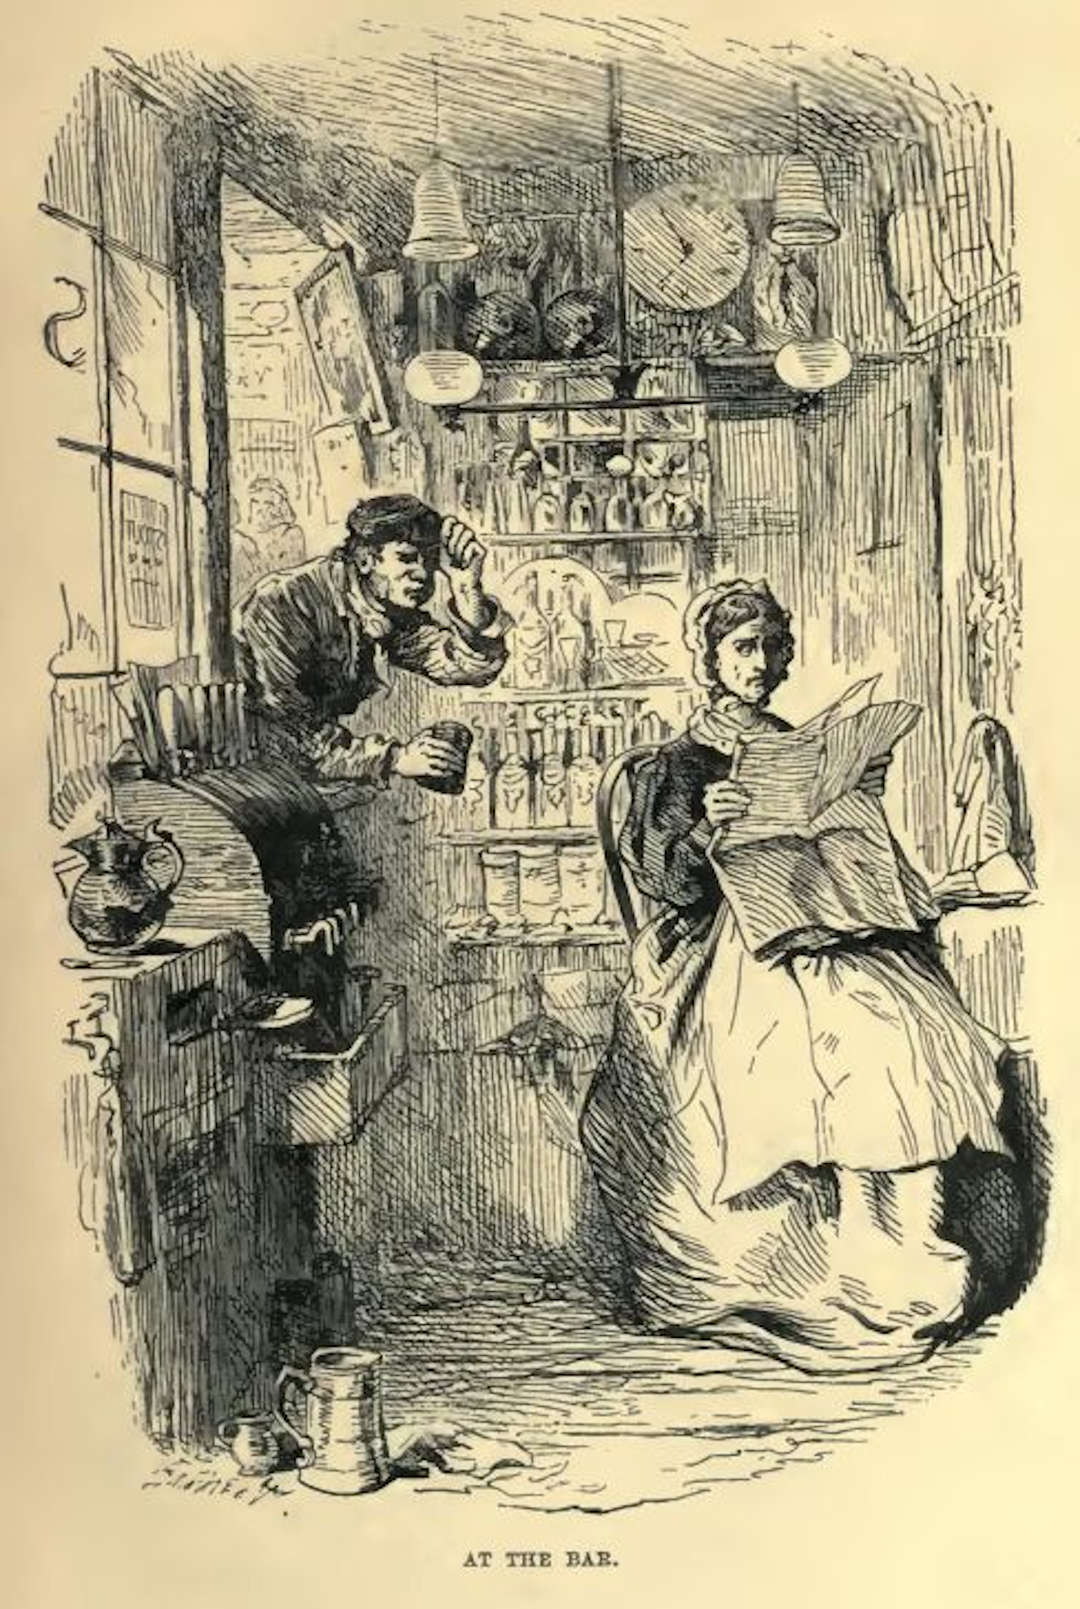
\includegraphics[scale=2.3]{01-06-01}

‘Certainly,’ said Miss Potterson.

‘Is it that you’re afraid of--’

‘I am not afraid OF YOU,’ interposed Miss Potterson, ‘if you mean that.’

‘But I humbly don’t mean that, Miss Abbey.’

‘Then what do you mean?’

‘You really are so cruel hard upon me! What I was going to make
inquiries was no more than, might you have any apprehensions--leastways
beliefs or suppositions--that the company’s property mightn’t be
altogether to be considered safe, if I used the house too regular?’

‘What do you want to know for?’

‘Well, Miss Abbey, respectfully meaning no offence to you, it would
be some satisfaction to a man’s mind, to understand why the Fellowship
Porters is not to be free to such as me, and is to be free to such as
Gaffer.’

The face of the hostess darkened with some shadow of perplexity, as she
replied: ‘Gaffer has never been where you have been.’

‘Signifying in Quod, Miss? Perhaps not. But he may have merited it. He
may be suspected of far worse than ever I was.’

‘Who suspects him?’

‘Many, perhaps. One, beyond all doubts. I do.’

‘YOU are not much,’ said Miss Abbey Potterson, knitting her brows again
with disdain.

‘But I was his pardner. Mind you, Miss Abbey, I was his pardner. As
such I know more of the ins and outs of him than any person living does.
Notice this! I am the man that was his pardner, and I am the man that
suspects him.’

‘Then,’ suggested Miss Abbey, though with a deeper shade of perplexity
than before, ‘you criminate yourself.’

‘No I don’t, Miss Abbey. For how does it stand? It stands this way. When
I was his pardner, I couldn’t never give him satisfaction. Why couldn’t
I never give him satisfaction? Because my luck was bad; because I
couldn’t find many enough of ‘em. How was his luck? Always good. Notice
this! Always good! Ah! There’s a many games, Miss Abbey, in which
there’s chance, but there’s a many others in which there’s skill too,
mixed along with it.’

‘That Gaffer has a skill in finding what he finds, who doubts, man?’
asked Miss Abbey.

‘A skill in purwiding what he finds, perhaps,’ said Riderhood, shaking
his evil head.

Miss Abbey knitted her brow at him, as he darkly leered at her. ‘If
you’re out upon the river pretty nigh every tide, and if you want to
find a man or woman in the river, you’ll greatly help your luck, Miss
Abbey, by knocking a man or woman on the head aforehand and pitching ‘em
in.’

‘Gracious Lud!’ was the involuntary exclamation of Miss Potterson.

‘Mind you!’ returned the other, stretching forward over the half door
to throw his words into the bar; for his voice was as if the head of his
boat’s mop were down his throat; ‘I say so, Miss Abbey! And mind you!
I’ll follow him up, Miss Abbey! And mind you! I’ll bring him to hook at
last, if it’s twenty year hence, I will! Who’s he, to be favoured along
of his daughter? Ain’t I got a daughter of my own!’

With that flourish, and seeming to have talked himself rather more drunk
and much more ferocious than he had begun by being, Mr Riderhood took up
his pint pot and swaggered off to the taproom.

Gaffer was not there, but a pretty strong muster of Miss Abbey’s pupils
were, who exhibited, when occasion required, the greatest docility. On
the clock’s striking ten, and Miss Abbey’s appearing at the door, and
addressing a certain person in a faded scarlet jacket, with ‘George
Jones, your time’s up! I told your wife you should be punctual,’
Jones submissively rose, gave the company good-night, and retired. At
half-past ten, on Miss Abbey’s looking in again, and saying, ‘William
Williams, Bob Glamour, and Jonathan, you are all due,’ Williams, Bob,
and Jonathan with similar meekness took their leave and evaporated.
Greater wonder than these, when a bottle-nosed person in a glazed hat
had after some considerable hesitation ordered another glass of gin and
water of the attendant potboy, and when Miss Abbey, instead of sending
it, appeared in person, saying, ‘Captain Joey, you have had as much as
will do you good,’ not only did the captain feebly rub his knees and
contemplate the fire without offering a word of protest, but the rest
of the company murmured, ‘Ay, ay, Captain! Miss Abbey’s right; you
be guided by Miss Abbey, Captain.’ Nor, was Miss Abbey’s vigilance in
anywise abated by this submission, but rather sharpened; for, looking
round on the deferential faces of her school, and descrying two other
young persons in need of admonition, she thus bestowed it: ‘Tom Tootle,
it’s time for a young fellow who’s going to be married next month, to
be at home and asleep. And you needn’t nudge him, Mr Jack Mullins, for
I know your work begins early tomorrow, and I say the same to you.
So come! Good-night, like good lads!’ Upon which, the blushing Tootle
looked to Mullins, and the blushing Mullins looked to Tootle, on the
question who should rise first, and finally both rose together and went
out on the broad grin, followed by Miss Abbey; in whose presence the
company did not take the liberty of grinning likewise.

In such an establishment, the white-aproned pot-boy with his
shirt-sleeves arranged in a tight roll on each bare shoulder, was a mere
hint of the possibility of physical force, thrown out as a matter of
state and form. Exactly at the closing hour, all the guests who were
left, filed out in the best order: Miss Abbey standing at the half door
of the bar, to hold a ceremony of review and dismissal. All wished
Miss Abbey good-night and Miss Abbey wished good-night to all, except
Riderhood. The sapient pot-boy, looking on officially, then had the
conviction borne in upon his soul, that the man was evermore outcast and
excommunicate from the Six Jolly Fellowship Porters.

‘You Bob Gliddery,’ said Miss Abbey to this pot-boy, ‘run round to
Hexam’s and tell his daughter Lizzie that I want to speak to her.’

With exemplary swiftness Bob Gliddery departed, and returned. Lizzie,
following him, arrived as one of the two female domestics of the
Fellowship Porters arranged on the snug little table by the bar fire,
Miss Potterson’s supper of hot sausages and mashed potatoes.

‘Come in and sit ye down, girl,’ said Miss Abbey. ‘Can you eat a bit?’

‘No thank you, Miss. I have had my supper.’

‘I have had mine too, I think,’ said Miss Abbey, pushing away the
untasted dish, ‘and more than enough of it. I am put out, Lizzie.’

‘I am very sorry for it, Miss.’

‘Then why, in the name of Goodness,’ quoth Miss Abbey, sharply, ‘do you
do it?’

‘I do it, Miss!’

‘There, there. Don’t look astonished. I ought to have begun with a word
of explanation, but it’s my way to make short cuts at things. I always
was a pepperer. You Bob Gliddery there, put the chain upon the door and
get ye down to your supper.’

With an alacrity that seemed no less referable to the pepperer fact
than to the supper fact, Bob obeyed, and his boots were heard descending
towards the bed of the river.

‘Lizzie Hexam, Lizzie Hexam,’ then began Miss Potterson, ‘how often have
I held out to you the opportunity of getting clear of your father, and
doing well?’

‘Very often, Miss.’

‘Very often? Yes! And I might as well have spoken to the iron funnel of
the strongest sea-going steamer that passes the Fellowship Porters.’

‘No, Miss,’ Lizzie pleaded; ‘because that would not be thankful, and I
am.’

‘I vow and declare I am half ashamed of myself for taking such an
interest in you,’ said Miss Abbey, pettishly, ‘for I don’t believe I
should do it if you were not good-looking. Why ain’t you ugly?’

Lizzie merely answered this difficult question with an apologetic
glance.

‘However, you ain’t,’ resumed Miss Potterson, ‘so it’s no use going into
that. I must take you as I find you. Which indeed is what I’ve done. And
you mean to say you are still obstinate?’

‘Not obstinate, Miss, I hope.’

‘Firm (I suppose you call it) then?’

‘Yes, Miss. Fixed like.’

‘Never was an obstinate person yet, who would own to the word!’ remarked
Miss Potterson, rubbing her vexed nose; ‘I’m sure I would, if I was
obstinate; but I am a pepperer, which is different. Lizzie Hexam, Lizzie
Hexam, think again. Do you know the worst of your father?’

‘Do I know the worst of father!’ she repeated, opening her eyes.

‘Do you know the suspicions to which your father makes himself liable?
Do you know the suspicions that are actually about, against him?’

The consciousness of what he habitually did, oppressed the girl heavily,
and she slowly cast down her eyes.

‘Say, Lizzie. Do you know?’ urged Miss Abbey.

‘Please to tell me what the suspicions are, Miss,’ she asked after a
silence, with her eyes upon the ground.

‘It’s not an easy thing to tell a daughter, but it must be told. It is
thought by some, then, that your father helps to their death a few of
those that he finds dead.’

The relief of hearing what she felt sure was a false suspicion, in place
of the expected real and true one, so lightened Lizzie’s breast for the
moment, that Miss Abbey was amazed at her demeanour. She raised her eyes
quickly, shook her head, and, in a kind of triumph, almost laughed.

‘They little know father who talk like that!’

[‘She takes it,’ thought Miss Abbey, ‘very quietly. She takes it with
extraordinary quietness!’)

‘And perhaps,’ said Lizzie, as a recollection flashed upon her, ‘it is
some one who has a grudge against father; some one who has threatened
father! Is it Riderhood, Miss?’

‘Well; yes it is.’

‘Yes! He was father’s partner, and father broke with him, and now he
revenges himself. Father broke with him when I was by, and he was very
angry at it. And besides, Miss Abbey!--Will you never, without strong
reason, let pass your lips what I am going to say?’

She bent forward to say it in a whisper.

‘I promise,’ said Miss Abbey.

‘It was on the night when the Harmon murder was found out, through
father, just above bridge. And just below bridge, as we were sculling
home, Riderhood crept out of the dark in his boat. And many and many
times afterwards, when such great pains were taken to come to the bottom
of the crime, and it never could be come near, I thought in my own
thoughts, could Riderhood himself have done the murder, and did he
purposely let father find the body? It seemed a’most wicked and cruel
to so much as think such a thing; but now that he tries to throw it upon
father, I go back to it as if it was a truth. Can it be a truth? That
was put into my mind by the dead?’

She asked this question, rather of the fire than of the hostess of the
Fellowship Porters, and looked round the little bar with troubled eyes.

But, Miss Potterson, as a ready schoolmistress accustomed to bring her
pupils to book, set the matter in a light that was essentially of this
world.

‘You poor deluded girl,’ she said, ‘don’t you see that you can’t open
your mind to particular suspicions of one of the two, without opening
your mind to general suspicions of the other? They had worked together.
Their goings-on had been going on for some time. Even granting that it
was as you have had in your thoughts, what the two had done together
would come familiar to the mind of one.’

‘You don’t know father, Miss, when you talk like that. Indeed, indeed,
you don’t know father.’

‘Lizzie, Lizzie,’ said Miss Potterson. ‘Leave him. You needn’t break
with him altogether, but leave him. Do well away from him; not because
of what I have told you to-night--we’ll pass no judgment upon that,
and we’ll hope it may not be--but because of what I have urged on you
before. No matter whether it’s owing to your good looks or not, I like
you and I want to serve you. Lizzie, come under my direction. Don’t
fling yourself away, my girl, but be persuaded into being respectable
and happy.’

In the sound good feeling and good sense of her entreaty, Miss Abbey
had softened into a soothing tone, and had even drawn her arm round the
girl’s waist. But, she only replied, ‘Thank you, thank you! I can’t. I
won’t. I must not think of it. The harder father is borne upon, the more
he needs me to lean on.’

And then Miss Abbey, who, like all hard people when they do soften,
felt that there was considerable compensation owing to her, underwent
reaction and became frigid.

‘I have done what I can,’ she said, ‘and you must go your way. You make
your bed, and you must lie on it. But tell your father one thing: he
must not come here any more.’

‘Oh, Miss, will you forbid him the house where I know he’s safe?’

‘The Fellowships,’ returned Miss Abbey, ‘has itself to look to, as well
as others. It has been hard work to establish order here, and make the
Fellowships what it is, and it is daily and nightly hard work to keep it
so. The Fellowships must not have a taint upon it that may give it a bad
name. I forbid the house to Riderhood, and I forbid the house to Gaffer.
I forbid both, equally. I find from Riderhood and you together, that
there are suspicions against both men, and I’m not going to take upon
myself to decide betwixt them. They are both tarred with a dirty brush,
and I can’t have the Fellowships tarred with the same brush. That’s all
I know.’

‘Good-night, Miss!’ said Lizzie Hexam, sorrowfully.

‘Hah!--Good-night!’ returned Miss Abbey with a shake of her head.

‘Believe me, Miss Abbey, I am truly grateful all the same.’

‘I can believe a good deal,’ returned the stately Abbey, ‘so I’ll try to
believe that too, Lizzie.’

No supper did Miss Potterson take that night, and only half her usual
tumbler of hot Port Negus. And the female domestics--two robust sisters,
with staring black eyes, shining flat red faces, blunt noses, and strong
black curls, like dolls--interchanged the sentiment that Missis had had
her hair combed the wrong way by somebody. And the pot-boy afterwards
remarked, that he hadn’t been ‘so rattled to bed’, since his late mother
had systematically accelerated his retirement to rest with a poker.

The chaining of the door behind her, as she went forth, disenchanted
Lizzie Hexam of that first relief she had felt. The night was black and
shrill, the river-side wilderness was melancholy, and there was a sound
of casting-out, in the rattling of the iron-links, and the grating of
the bolts and staples under Miss Abbey’s hand. As she came beneath
the lowering sky, a sense of being involved in a murky shade of Murder
dropped upon her; and, as the tidal swell of the river broke at her feet
without her seeing how it gathered, so, her thoughts startled her by
rushing out of an unseen void and striking at her heart.

Of her father’s being groundlessly suspected, she felt sure. Sure. Sure.
And yet, repeat the word inwardly as often as she would, the attempt to
reason out and prove that she was sure, always came after it and failed.
Riderhood had done the deed, and entrapped her father. Riderhood had
not done the deed, but had resolved in his malice to turn against her
father, the appearances that were ready to his hand to distort. Equally
and swiftly upon either putting of the case, followed the frightful
possibility that her father, being innocent, yet might come to be
believed guilty. She had heard of people suffering Death for bloodshed
of which they were afterwards proved pure, and those ill-fated persons
were not, first, in that dangerous wrong in which her father stood. Then
at the best, the beginning of his being set apart, whispered against,
and avoided, was a certain fact. It dated from that very night. And as
the great black river with its dreary shores was soon lost to her view
in the gloom, so, she stood on the river’s brink unable to see into the
vast blank misery of a life suspected, and fallen away from by good and
bad, but knowing that it lay there dim before her, stretching away to
the great ocean, Death.

One thing only, was clear to the girl’s mind. Accustomed from her very
babyhood promptly to do the thing that could be done--whether to keep
out weather, to ward off cold, to postpone hunger, or what not--she
started out of her meditation, and ran home.

The room was quiet, and the lamp burnt on the table. In the bunk in the
corner, her brother lay asleep. She bent over him softly, kissed him,
and came to the table.

‘By the time of Miss Abbey’s closing, and by the run of the tide, it
must be one. Tide’s running up. Father at Chiswick, wouldn’t think of
coming down, till after the turn, and that’s at half after four. I’ll
call Charley at six. I shall hear the church-clocks strike, as I sit
here.’

Very quietly, she placed a chair before the scanty fire, and sat down in
it, drawing her shawl about her.

‘Charley’s hollow down by the flare is not there now. Poor Charley!’

The clock struck two, and the clock struck three, and the clock struck
four, and she remained there, with a woman’s patience and her own
purpose. When the morning was well on between four and five, she slipped
off her shoes (that her going about might not wake Charley), trimmed
the fire sparingly, put water on to boil, and set the table for
breakfast. Then she went up the ladder, lamp in hand, and came down
again, and glided about and about, making a little bundle. Lastly, from
her pocket, and from the chimney-piece, and from an inverted basin
on the highest shelf she brought halfpence, a few sixpences, fewer
shillings, and fell to laboriously and noiselessly counting them, and
setting aside one little heap. She was still so engaged, when she was
startled by:

‘Hal-loa!’ From her brother, sitting up in bed.

‘You made me jump, Charley.’

‘Jump! Didn’t you make ME jump, when I opened my eyes a moment ago, and
saw you sitting there, like the ghost of a girl miser, in the dead of
the night.’

‘It’s not the dead of the night, Charley. It’s nigh six in the morning.’

‘Is it though? But what are you up to, Liz?’

‘Still telling your fortune, Charley.’

‘It seems to be a precious small one, if that’s it,’ said the boy. ‘What
are you putting that little pile of money by itself for?’

‘For you, Charley.’

‘What do you mean?’

‘Get out of bed, Charley, and get washed and dressed, and then I’ll tell
you.’

Her composed manner, and her low distinct voice, always had an influence
over him. His head was soon in a basin of water, and out of it again,
and staring at her through a storm of towelling.

‘I never,’ towelling at himself as if he were his bitterest enemy, ‘saw
such a girl as you are. What IS the move, Liz?’

‘Are you almost ready for breakfast, Charley?’

‘You can pour it out. Hal-loa! I say? And a bundle?’

‘And a bundle, Charley.’

‘You don’t mean it’s for me, too?’

‘Yes, Charley; I do; indeed.’

More serious of face, and more slow of action, than he had been, the
boy completed his dressing, and came and sat down at the little
breakfast-table, with his eyes amazedly directed to her face.

‘You see, Charley dear, I have made up my mind that this is the right
time for your going away from us. Over and above all the blessed change
of by-and-bye, you’ll be much happier, and do much better, even so soon
as next month. Even so soon as next week.’

‘How do you know I shall?’

‘I don’t quite know how, Charley, but I do.’ In spite of her unchanged
manner of speaking, and her unchanged appearance of composure, she
scarcely trusted herself to look at him, but kept her eyes employed on
the cutting and buttering of his bread, and on the mixing of his tea,
and other such little preparations. ‘You must leave father to me,
Charley--I will do what I can with him--but you must go.’

‘You don’t stand upon ceremony, I think,’ grumbled the boy, throwing his
bread and butter about, in an ill-humour.

She made him no answer.

‘I tell you what,’ said the boy, then, bursting out into an angry
whimpering, ‘you’re a selfish jade, and you think there’s not enough for
three of us, and you want to get rid of me.’

‘If you believe so, Charley,--yes, then I believe too, that I am a
selfish jade, and that I think there’s not enough for three of us, and
that I want to get rid of you.’

It was only when the boy rushed at her, and threw his arms round her
neck, that she lost her self-restraint. But she lost it then, and wept
over him.

‘Don’t cry, don’t cry! I am satisfied to go, Liz; I am satisfied to go.
I know you send me away for my good.’

‘O, Charley, Charley, Heaven above us knows I do!’

‘Yes yes. Don’t mind what I said. Don’t remember it. Kiss me.’

After a silence, she loosed him, to dry her eyes and regain her strong
quiet influence.

‘Now listen, Charley dear. We both know it must be done, and I alone
know there is good reason for its being done at once. Go straight to the
school, and say that you and I agreed upon it--that we can’t overcome
father’s opposition--that father will never trouble them, but will never
take you back. You are a credit to the school, and you will be a greater
credit to it yet, and they will help you to get a living. Show what
clothes you have brought, and what money, and say that I will send some
more money. If I can get some in no other way, I will ask a little help
of those two gentlemen who came here that night.’

‘I say!’ cried her brother, quickly. ‘Don’t you have it of that chap
that took hold of me by the chin! Don’t you have it of that Wrayburn
one!’

Perhaps a slight additional tinge of red flushed up into her face and
brow, as with a nod she laid a hand upon his lips to keep him silently
attentive.

‘And above all things mind this, Charley! Be sure you always speak well
of father. Be sure you always give father his full due. You can’t deny
that because father has no learning himself he is set against it in
you; but favour nothing else against him, and be sure you say--as you
know--that your sister is devoted to him. And if you should ever happen
to hear anything said against father that is new to you, it will not be
true. Remember, Charley! It will not be true.’

The boy looked at her with some doubt and surprise, but she went on
again without heeding it.

‘Above all things remember! It will not be true. I have nothing more to
say, Charley dear, except, be good, and get learning, and only think of
some things in the old life here, as if you had dreamed them in a dream
last night. Good-bye, my Darling!’

Though so young, she infused in these parting words a love that was far
more like a mother’s than a sister’s, and before which the boy was quite
bowed down. After holding her to his breast with a passionate cry, he
took up his bundle and darted out at the door, with an arm across his
eyes.

The white face of the winter day came sluggishly on, veiled in a
frosty mist; and the shadowy ships in the river slowly changed to black
substances; and the sun, blood-red on the eastern marshes behind dark
masts and yards, seemed filled with the ruins of a forest it had set on
fire. Lizzie, looking for her father, saw him coming, and stood upon the
causeway that he might see her.

He had nothing with him but his boat, and came on apace. A knot of those
amphibious human-creatures who appear to have some mysterious power
of extracting a subsistence out of tidal water by looking at it, were
gathered together about the causeway. As her father’s boat grounded,
they became contemplative of the mud, and dispersed themselves. She saw
that the mute avoidance had begun.

Gaffer saw it, too, in so far as that he was moved when he set foot on
shore, to stare around him. But, he promptly set to work to haul up his
boat, and make her fast, and take the sculls and rudder and rope out of
her. Carrying these with Lizzie’s aid, he passed up to his dwelling.

‘Sit close to the fire, father, dear, while I cook your breakfast.
It’s all ready for cooking, and only been waiting for you. You must be
frozen.’

‘Well, Lizzie, I ain’t of a glow; that’s certain. And my hands seem
nailed through to the sculls. See how dead they are!’ Something
suggestive in their colour, and perhaps in her face, struck him as he
held them up; he turned his shoulder and held them down to the fire.

‘You were not out in the perishing night, I hope, father?’

‘No, my dear. Lay aboard a barge, by a blazing coal-fire.--Where’s that
boy?’

‘There’s a drop of brandy for your tea, father, if you’ll put it in
while I turn this bit of meat. If the river was to get frozen, there
would be a deal of distress; wouldn’t there, father?’

‘Ah! there’s always enough of that,’ said Gaffer, dropping the liquor
into his cup from a squat black bottle, and dropping it slowly that it
might seem more; ‘distress is for ever a going about, like sut in the
air--Ain’t that boy up yet?’

‘The meat’s ready now, father. Eat it while it’s hot and comfortable.
After you have finished, we’ll turn round to the fire and talk.’

But, he perceived that he was evaded, and, having thrown a hasty angry
glance towards the bunk, plucked at a corner of her apron and asked:

‘What’s gone with that boy?’

‘Father, if you’ll begin your breakfast, I’ll sit by and tell you.’ He
looked at her, stirred his tea and took two or three gulps, then cut at
his piece of hot steak with his case-knife, and said, eating:

‘Now then. What’s gone with that boy?’

‘Don’t be angry, dear. It seems, father, that he has quite a gift of
learning.’

‘Unnat’ral young beggar!’ said the parent, shaking his knife in the air.

‘And that having this gift, and not being equally good at other things,
he has made shift to get some schooling.’

‘Unnat’ral young beggar!’ said the parent again, with his former action.

‘--And that knowing you have nothing to spare, father, and not wishing
to be a burden on you, he gradually made up his mind to go seek his
fortune out of learning. He went away this morning, father, and he cried
very much at going, and he hoped you would forgive him.’

‘Let him never come a nigh me to ask me my forgiveness,’ said the
father, again emphasizing his words with the knife. ‘Let him never come
within sight of my eyes, nor yet within reach of my arm. His own father
ain’t good enough for him. He’s disowned his own father. His own father
therefore, disowns him for ever and ever, as a unnat’ral young beggar.’

He had pushed away his plate. With the natural need of a strong rough
man in anger, to do something forcible, he now clutched his knife
overhand, and struck downward with it at the end of every succeeding
sentence. As he would have struck with his own clenched fist if there
had chanced to be nothing in it.

‘He’s welcome to go. He’s more welcome to go than to stay. But let him
never come back. Let him never put his head inside that door. And let
you never speak a word more in his favour, or you’ll disown your own
father, likewise, and what your father says of him he’ll have to come to
say of you. Now I see why them men yonder held aloof from me. They says
to one another, “Here comes the man as ain’t good enough for his own
son!” Lizzie--!’

But, she stopped him with a cry. Looking at her he saw her, with a face
quite strange to him, shrinking back against the wall, with her hands
before her eyes.

‘Father, don’t! I can’t bear to see you striking with it. Put it down!’

He looked at the knife; but in his astonishment still held it.

‘Father, it’s too horrible. O put it down, put it down!’

Confounded by her appearance and exclamation, he tossed it away, and
stood up with his open hands held out before him.

‘What’s come to you, Liz? Can you think I would strike at you with a
knife?’

‘No, father, no; you would never hurt me.’

‘What should I hurt?’

‘Nothing, dear father. On my knees, I am certain, in my heart and soul
I am certain, nothing! But it was too dreadful to bear; for it looked--’
her hands covering her face again, ‘O it looked--’

‘What did it look like?’

The recollection of his murderous figure, combining with her trial of
last night, and her trial of the morning, caused her to drop at his
feet, without having answered.

He had never seen her so before. He raised her with the utmost
tenderness, calling her the best of daughters, and ‘my poor pretty
creetur’, and laid her head upon his knee, and tried to restore her. But
failing, he laid her head gently down again, got a pillow and placed it
under her dark hair, and sought on the table for a spoonful of brandy.
There being none left, he hurriedly caught up the empty bottle, and ran
out at the door.

He returned as hurriedly as he had gone, with the bottle still empty.
He kneeled down by her, took her head on his arm, and moistened her lips
with a little water into which he dipped his fingers: saying, fiercely,
as he looked around, now over this shoulder, now over that:

‘Have we got a pest in the house? Is there summ’at deadly sticking to my
clothes? What’s let loose upon us? Who loosed it?’




{\LARGE (TO BE CONTINUED)}

\chapter*{Disclaimer}
This eBook may be freely used in the United States because it is not protected by U.S. copyright law.
They may not be free of copyright in other countries.
Readers outside of the United States must check the copyright terms of their countries before accessing,
downloading or redistributing this eBook.

This \LaTeX ebook is just humorous intention of fighting the lockdown boredom.
My apology to Sir Paul McCartney and Charles Dickens.

% %%%%%%%%%%%%
\end{document}%
% End of document.
% %%%%%%%%%%%%%%%%


